\documentclass[11pt,fancychapters]{report}
\usepackage[a4paper, total={6in, 8in}]{geometry}
\usepackage{listings}
\usepackage{color}
\usepackage{setspace}
\usepackage{hyperref}
\usepackage{acro}
\usepackage{amsmath}
\usepackage{amsthm}
\usepackage{amssymb}
\usepackage{amsfonts}
\usepackage{graphicx}
\usepackage{geometry}
\usepackage{cancel}
\usepackage{tikz}
\usepackage{subcaption}
\usepackage{bm}
\usetikzlibrary{calc,trees,positioning,arrows,chains,shapes.geometric,%
    decorations.pathreplacing,decorations.pathmorphing,shapes,%
    matrix,shapes.symbols}
\DeclareAcronym{etf}{
	short = ETF,
    long = Exchange-Traded Fund,
    class = abbrev
}

\DeclareAcronym{aum}{
	short = AUM,
    long = Assets Under Management,
    class = abbrev
}

\DeclareAcronym{sr}{
	short = SR,
    long = Sharpe Ratio,
    class = abbrev
}

\DeclareAcronym{nyse}{
	short = NYSE,
    long = New York Stock Exchange,
    class = abbrev
}

\DeclareAcronym{hft}{
	short = HFT,
    long = High Frequency Trading,
    class = abbrev
}

\DeclareAcronym{pv}{
	short = PV,
    long = present value,
    class = abbrev
}

\DeclareAcronym{fv}{
	short = FV,
    long = future value,
    class = abbrev
}

\DeclareAcronym{ir}{
	short = IR,
    long = interest rate,
    class = abbrev
}

\DeclareAcronym{capm}{
	short = CAPM,
    long = Capital Assets Pricing Model,
    class = abbrev
}

\DeclareAcronym{apt}{
	short = APT,
    long = Arbitrage Pricing Theory,
    class = abbrev
}

\DeclareAcronym{sma}{
	short = SMA,
    long = simple moving average,
    class = abbrev
}

\DeclareAcronym{mvo}{
	short = MVO,
    long = mean variance optimization,
    class = abbrev
}

\DeclareAcronym{rmse}{
	short = RMSE,
    long = root mean square error,
    class = abbrev
}

\DeclareAcronym{kNN}{
	short = kNN,
    long = k-nearest neighbor,
    class = abbrev
}
\geometry{top=1.3in,bottom=1.3in}
\hypersetup{
    colorlinks,
    citecolor=black,
    filecolor=black,
    linkcolor=black,
    urlcolor=black
}

\DeclareMathOperator*{\argmin}{arg\,min}

\DeclareMathOperator*{\argmax}{arg\,max}

\setcounter{secnumdepth}{4}

\definecolor{DarkerGreen}{RGB}{0,179,45}

\definecolor{Code}{rgb}{0,0,0}
\definecolor{Decorators}{rgb}{0.5,0.5,0.5}
\definecolor{Numbers}{rgb}{0.5,0,0}
\definecolor{MatchingBrackets}{rgb}{0.25,0.5,0.5}
\definecolor{Keywords}{rgb}{0,0,1}
\definecolor{self}{rgb}{0,0,0}
\definecolor{Strings}{rgb}{0,0.63,0}
\definecolor{Comments}{rgb}{0,0.63,1}
\definecolor{Backquotes}{rgb}{0,0,0}
\definecolor{Classname}{rgb}{0,0,0}
\definecolor{FunctionName}{rgb}{0,0,.7}
\definecolor{Operators}{rgb}{0,0,0}
\definecolor{Background}{rgb}{0.98,0.98,0.98}

\lstdefinestyle{python}{
  numbers=left,
  numberstyle=\footnotesize,
  numbersep=1em,
  xleftmargin=1em,
  framextopmargin=2em,
  framexbottommargin=2em,
  showspaces=false,
  showtabs=false,
  showstringspaces=false,
  frame=l,
  tabsize=4,
  % Basic
  basicstyle=\ttfamily\small\setstretch{1},
  backgroundcolor=\color{Background},
  language=Python,
  % Comments
  commentstyle=\color{Comments}\slshape,
  % Strings
  stringstyle=\color{Strings},
  morecomment=[s][\color{Strings}]{"""}{"""},
  morecomment=[s][\color{Strings}]{'''}{'''},
  % keywords
  morekeywords={import,from,class,def,for,while,if,is,in,elif,else,not,and,or,print,break,continue,return,True,False,None,access,as,,del,except,exec,finally,global,import,lambda,pass,print,raise,try,assert},
  keywordstyle={\color{Keywords}\bfseries},
  % additional keywords
  morekeywords={[2]@invariant},
  keywordstyle={[2]\color{Decorators}\slshape},
  emph={self},
  emphstyle={\color{self}\slshape},
  breaklines=true
}
\addcontentsline{toc}{chapter}{Preface}

\newtheorem{exmp}{Example}[section]

\newcommand{\codeExample}[2]{
	\begin{exmp}
      #1
      \noindent\begin{minipage}{\linewidth}
      \begin{lstlisting}[style=python]
          #2
      \end{lstlisting}
      \end{minipage}
    \end{exmp}
}

\newcommand\MyLBrace[2]{%
  \left.\rule{0pt}{#1}\right\}\text{#2}}
  
\tikzset{
>=stealth',
  punktchain/.style={
    rectangle, 
    rounded corners, 
    % fill=black!10,
    draw=black, very thick,
    text width=10em, 
    minimum height=3em, 
    text centered, 
    on chain},
  line/.style={draw, thick, <-},
  element/.style={
    tape,
    top color=white,
    bottom color=blue!50!black!60!,
    minimum width=8em,
    draw=blue!40!black!90, very thick,
    text width=10em, 
    minimum height=3.5em, 
    text centered, 
    on chain},
  every join/.style={->, thick,shorten >=1pt},
  decoration={brace},
  tuborg/.style={decorate},
  tubnode/.style={midway, right=2pt},
}

\title{Intelligence}
\author{Joseph Marino}

\begin{document}

\maketitle
\pagenumbering{gobble}
\newpage
\pagenumbering{roman}
\tableofcontents
\newpage
\pagenumbering{arabic}

\chapter*{Preface}

Despite advances in our understanding of computation in both biological and artificial systems, we are still far from comprehending the mechanisms of biological intelligence or how to build intelligent machine systems. This manuscript is an attempt to collect and synthesize our current knowledge in these areas, so as to facilitate further progress.

\part{Introduction}
\chapter{Intelligence}

\section{Defining Intelligence}

The purpose of this manuscript is to build a common base of knowledge for understanding \textit{intelligence} across all systems, both biological and non-biological. To understand what makes a system intelligent, we must first define intelligence. Intelligence is a fuzzy term that carries many varying connotations. Our everyday notion of intelligence fails to objectively capture this attribute in the most general sense of the term.

Let's start by stating that intelligence is the property of a \textit{system}, which we define as a collection of matter. Systems can exist on different scales and can be composed: 

\begin{center}
	\textbf{Intelligence} is the ability of a system to convert energy into work to alter the trajectory of the universe. 
\end{center}

Consider the concepts of \textit{matter}, \textit{state}, and \textit{energy}. Matter, here, is the normal, everyday matter that we encounter, which is composed of atoms. The state defines the configuration of the matter, consisting of the location and motion of every atom. Energy is a more difficult concept, that 


Under certain conditions, a \textit{system}, composed of matter, can convert energy into work. This allows the system to alter its own state, as well as the state of the matter in the surrounding \textit{environment}. We can then ask which states can and cannot be reached as a result of the work performed. It is precisely the ability to reach a particular state, or set of states, that we define as \textit{intelligence}. In this sense, intelligence is only defined in the context of a state transition. If a system can achieve a given state transition, which we refer to as a \textit{task}, then it is intelligent with respect to that task. While intelligence can be defined for any task, the main task that we find in naturally occurring systems is reproduction. Tautologically, a system that is unable to reproduce (or survive indefinitely) will eventually be destroyed and no longer exist.



Let us start by stating that intelligence is the property of a \textit{system}. We restrict our discussion to the physical realm, where a system is defined as a collection of matter, such as a biological organism or a designed machine. However, more generally, the notion of a system could also be applied within abstract or virtual worlds. 

\textit{Need to define intelligence. Need to first discuss basics of energy and entropy.}

Note that very few physical systems are intelligent. Beyond our planet, it seems that the universe is not conducive for intelligent systems. 

\subsection{Maxwell's ``Demon"}

Maxwell's demon is the simplest example of an intelligent system....?

Some definitions of intelligence from AIXI: \cite{legg2007universal}

Douglas Hofstadter's \cite{hofstadter1980godel} essential abilities of an intelligent system (reproduced):
\begin{itemize}
    \item to respond to situations very flexibly;
    \item to take advantage of fortuitous circumstances;
    \item to make sense out of ambiguous or contradictory messages;
    \item to recognize the relative importance of different elements of a situation;
    \item to find similarities between situations despite differences which may separate them;
    \item to draw distinctions between situations despite similarities which may link them;
    \item to synthesize new concepts by taking old concepts and putting them together in new ways;
    \item to come up with ideas which are novel.
\end{itemize}

I define intelligence as follows:

Intelligence is a quality that must be measured. It does not exist in a vacuum, independent from an external environment. The only way in which to measure the intelligence of a system is through its ability to solve tasks, which depends on the system's outputs within the environment. Intelligence is not one particular thing, but rather a \textit{space} with a multitude of dimensions. As it is defined according to solving tasks, a system can be intelligent with regards to some tasks but not others. It is also important to note that solving a task may not be an all-or-none phenomenon. A system may be able to solve a task to a certain percentage of success and it would still be considered intelligent.

The notion of solving tasks gets at the deeper concept of environmental \textit{states}. The surrounding environment of an intelligent system can be in an infinite number of underlying states. Considering every possible arrangement of matter, most of these states will be highly disordered. The second law of thermodynamics dictates that the state of the environment will tend toward these disordered states, as they are more probable. In other words, entropy tends to increase overall. \textbf{``Solving a task" denotes arriving at some environmental state or set of states (a macro-state).} The probability of the state, in some sense, then defines the difficulty of the task. 

As an example, say that your task is to be at the other end of the room. In the entire universe, ``you at the other end of the room" defines an infinite set of states. However, there are \textit{infinitely many more} states where you are not at the other end of the room, and according to Newton's first law, you will stay where you are unless acted on by a force. Without a force, it is therefore improbable that the state of the environment will be one in which you are at the other end of the room. But because you are a system that is built to solve this task, you can arrive at this improbable environmental macro-state.

The task for natural, biological systems is clear: \textbf{survive}, ideally long enough to reproduce and ensure the survival of the offspring. Survival is indeed the \textit{only} task for intelligent systems in the natural world, as it is the only task that results in persisting intelligent systems. An intelligent system that is not capable of surviving is eventually destroyed, again, due to the second law of thermodynamics. There are infinitely many states that consist of a system's survival, but there are infinitely many more states that consist of a system's demise. As such, we observe systems in the natural world that are highly specialized to ensure their own survival.

A key question in creating intelligent machines will be what tasks they are expected to perform. While biological systems are built for survival, this need not be the case for any arbitrary intelligent system. Of course, we will likely create machines that are capable of ensuring their own survival, as this is more cost-effective and less wasteful. It is just important to point out that this is not necessarily the default operating mode. We could just as easily create intelligent machines that have no preference for their own survival. Intelligent systems are also not inherently good or evil. It is the tasks that they are built to perform that determine their actions. Coming up with the desired set of tasks and specifying these tasks clearly is an important consideration for building intelligent machines.

Intelligence is also not unique to contiguous collections of matter. Intelligence can be a property of systems more generally. The many devices that we have created assist in augmenting our intelligence. For instance, with a car, we can travel long distances in short amounts of time. Neither the car nor the person can do this on its own. Rather, the car-person system as a whole possesses the intelligence. Likewise, groups of people can be intelligent in ways beyond any single person. No one person constructs a skyscraper or sends people to the moon. It is the group system that is able to solve those tasks; it is the group system that is intelligent. This is relevant, as it highlights that we should not restrict intelligence to a measure of a single entity. A non-biological intelligent system can be much more than one standalone machine.



\section{Intelligent Systems Perform Work}

Work processes, both in biological and non-biological systems, require energy. Through converting energy into useful work, such systems bring about change, both to the system itself, as well as the environment in which the system interacts. Importantly, work comes in many forms, and in biological systems, work can be studied at many hierarchical levels. To understand work, we must first understand energy through the laws of thermodynamics:
\begin{enumerate}
    \item \textbf{First Law of Thermodynamics}: Energy cannot be created or destroyed; it is conserved. However, energy can be transformed from one form into another. This conversion process is called \textit{energy transduction}, and is an important process in biological and non-biological systems. The first law does not specify how work is converted, but does specify a \textit{performance envelope} dictating how much work a system can perform.
    
    \item \textbf{Second Law of Thermodynamics}: Roughly, order in the universe is, on average, constantly decreasing. Thus, for a highly ordered system to exist, it must require a constant input of energy. This allows the system to oppose the tendency toward disorder by maintaining and repairing itself.
    
    \item \textbf{Third Law of Thermodynamics}: Temperature fundamentally characterizes how work gets done. It plays an important role in defining the performance envelope of a system. Thus, systems must often spend considerable energy maintaining their temperature, whether it be a biological organism or an office building.
\end{enumerate}

Through the process of energy transduction, a system can convert energy into \textit{potential energy}, which can then be converted into \textit{useful work}. For instance, one could use an energy input to pump water up a mountain, thereby converting the energy into potential energy. Using the flow of water down the mountain, one could convert this energy into the work of spinning a turbine. A similar work process is ubiquitous in biological systems.

\subsection{Cellular Work Processes in Biological Systems}

Energy is required to perform the work of sustaining the order within biological systems. How is this energy obtained and converted? In animals, energy comes from organic nutrients, such as glucose, which are the result of breaking down foods. In plants, energy is instead obtained from the sun through photosynthesis, then converted into organic nutrients. In biological systems, these organic nutrients are broken down step by step and carried through intermediate molecules, which then convert the energy into useful work. The main intermediate (or carrier) molecule in biological systems is ATP, adenosine triphosphate. Breaking down nutrients involves oxidation, which yields electrons. These electrons are used for \textit{proton pumping}, moving protons from one side of a cell membrane to the other. This creates a concentration gradient across the cell membrane. Using channels, which can harness the resulting flow of protons back across the membrane, the cell performs the work of ATP synthesis, combining adenosine diphosphate (ADP) and inorganic phosphate (P$_i$). This entire process is referred to as \textit{chemiosmosis}. ATP can then be converted into other forms of work, such as protein synthesis or muscular work. Chemiosmosis thus forms the foundation of work in biological systems, and cells are working constantly to maintain stockpiles of ATP. Note also that this process is highly temperature dependent. Chemiosmosis is highly conserved across all domains of biological organisms, and likely provided a fundamental step in further evolutionary development.


\section{The Future of Intelligence}

Predicting the future is notoriously difficult. Since the advent of computing machines, many experts have made wildly inaccurate predictions about intelligent machines. On the one hand, constructing a machine that is capable of behaving like a human seems so plausible, even obvious. On the other, we currently don't have the faintest idea of how our own intelligence works. \textbf{Intelligent machines are an obvious invention that we don't know how to build.} This ability to \textit{visualize} intelligent machines without \textit{realizing} them opens the door to speculation.

Rodney Brooks identifies seven deadly sins\footnote{https://rodneybrooks.com/the-seven-deadly-sins-of-predicting-the-future-of-ai/} of predicting the future of artificial intelligence. He starts by noting four areas in which there is hype and hysteria in the public:
\begin{itemize}
	\item \textbf{Artificial General Intelligence}: building general-purpose machines that can solve a variety of tasks, much in the same way that humans operate.
	\item \textbf{The Singularity}: the inflection point when intelligent machines start creating better intelligent machines.
	\item \textbf{Misaligned Values}: intelligent machines that interpret directions too literally or without common-sense understanding, going against our intentions.
	\item \textbf{``Evil" Intelligent Machines}: intelligent machines that purposefully destroy humans.
\end{itemize}
Brooks then goes on to identify seven deadly sins:
\begin{enumerate}
	\item \textbf{Over and Under Estimating}: We often have a difficult time estimating how a technology will play out. This is nicely summarized by Roy Amara's quote:
	
	\textit{We tend to overestimate the effect of a technology in the short run and underestimate the effect in the long run.}
	
	In other words, we often set too high of expectations upfront, then fail to estimate how impactful a technology will be down the road. Brooks gives the example of GPS, which took decades until it proved its usefulness, but it now an essential part of many aspects of society. 
	\item \textbf{Imagining Magic}: Future technologies are so far in the future that we simply do not have to ability to reason about their capabilities. This is encapsulated in Arthur C. Clark's third ``law":
	
	\textit{Any sufficiently advanced technology is indistinguishable from magic.}
	
	That is, reasoning about the capabilities of technologies in the distant future is somewhat like reasoning about magic; it's just not possible. Brooks gives the example of Isaac Newton being introduced to an iPhone. He would be astounded to see it producing light, capturing images, etc., and he would be unable to judge whether other capabilities, such as communicating with other people or transforming lead into gold, are reasonable.
	\item \textbf{Performance vs. Competence}: We are typically able to judge the \textit{competence} of humans based on their \textit{performance} on other tasks. For instance, if you can drive a manual transmission car, I should expect that you are also able to drive an automatic transmission car. These types of competence generalization assumptions do not hold up for machine systems, which we, as humans, find unintuitive.
	\item \textbf{Suitcase Words}: Marvin Minsky defines suitcase words as those that pack many different meanings, such as imagine, plan, reason, understand, recognize, and even learn. We are so accustomed to human intelligence that we tend to ascribe these words to intelligent machines, even when they only apply narrowly.
	\item \textbf{Exponentials}: People often use exponential trends to justify predictions about rapid progress in technology, particularly computing and intelligent machines. Brooks argues that Moore's Law is not a true ``law" and will not continue indefinitely. More broadly, technological exponential trends are often really just the start of an S-curve, and they tend to flatten out or fail for three reasons: (1) physical limits, (2) market demand, (3) they may not be exponential in the first place. Predicting the future of intelligent machines based on exponential trends is highly imprecise.
	\item \textbf{Hollywood Scenarios}: Many popular movies about intelligent machines in the future often picture these machines in our current technological landscape, often failing to imagine how other technologies will change. That is, there will be a series of technological innovations to get to wherever we end up; it will not be some sudden change.
	\item \textbf{Speed of Deployment}: The pace of deployment for hardware is much slower than that for software. This is due to higher capital costs, which places limits on the widespread adoption of technologies. Brooks identifies instances in factory automation technology and defense where technology is 20 to 50 years old and incredibly resistant to change. 
\end{enumerate}












\chapter{Embodied Intelligent Systems}
\label{chap: embodied intelligent systems}




\section{Task Specification}



\section{State Estimation}



\section{Control}



\part{Mathematics}
\chapter{Mathematical Basics}
\label{chap: mathematical basics}

\chapter{Probability \& Statistics}

Why define a system in terms of probability? Probability allows us to estimating uncertainty arising from stochasticity
\begin{itemize}
    \item in the system itself,
    \item in the measurement process, potentially the result of incomplete observability,
    \item due to limitations in the model, such as discretization.
\end{itemize}
There are two main interpretations of probability. The \textbf{frequentist} approach considers probabilities as the \textit{frequency} of events occurring, calculated over past trials. The \textbf{Bayesian} approach considers probabilities as a specifying the \textit{uncertainty} of events. Under the Bayesian interpretation, probability is a subjective belief, whereas under the frequentist interpretation, probability is an objective frequency of occurring events. While the basic rules of probability are consistent in both approaches, the advantage of the Bayesian approach is that it allows one to model uncertainty even when past trials have not necessarily been observed, providing flexibility. By expressing probability in terms of uncertainty, the Bayesian approach is also deeply connected to information theory (Chapter \ref{chap: information theory}), bringing additional mathematical tools for analysis. 

While probability gives us the tools to account for uncertainty in our estimates, it also brings a separate set of challenges associated with estimating various quantities. Rather than maintaining a single hypothesis about a quantity, probability often requires us to evaluate \textit{all} hypotheses. Instead of ``point estimates," we work with entire ``distributions." This creates computational difficulties stemming primarily from marginalization, i.e. summing or integrating over possible values. One common strategy for dealing with this is to forgo analytical estimates in favor of sampling-based estimates. In Chapter \ref{chap: variational inference}, we discuss variational inference, another technique for overcoming some of these issues.


\section{Probability}

Probabilities are defined for \textbf{random variables}, which can take either \textit{discrete} or \textit{continuous} values. A discrete variable could be whether or not a light switch is on, and a continuous variable could be the level of a light dimmer. A random variable only defines possible values that can be taken; to define the likelihood of the random variable taking each of the values, we must use a \textbf{probability distribution}. In the cases of the discrete and continuous random variables, the total probability of all values must sum to $1$ because the variable must take some value. The light switch must be on or off, and the light dimmer must be at some particular level. To accommodate this requirement, probabilities over discrete and continuous random variables must be handled differently, e.g. replacing summations with integrals, but the underlying rules of probability are identical in both cases.

\subsection{Discrete Random Variables}

Discrete random variables can take a finite or countably infinite number of values. Note that these values may not necessarily be numerical. In describing the probability over the values of a discrete random variable, we use a \textbf{probability mass function (PMF)}. A PMF, $P(x)$, is a function that maps discrete values of a random variable, $x$, to probabilities between $0$ and $1$, i.e.
$$\forall x, 0 \leq P(x) \leq 1. $$
Following our requirement that probability distributions must sum to $1$, we must ensure that
$$ \sum_x P(x) = 1. $$
We refer to a function meeting this requirement as being \textbf{normalized}. 

\subsection{Continuous Random Variables}

Continuous random variables take an uncountably infinite number of values, associated with a real value over some domain. To define the probability over this domain, we use a \textbf{probability density function (PDF)}. Unlike a PMF, a PDF, $p(x)$, is only required to be non-negative:
$$ \forall x, 0 \leq p(x). $$
Again, we must ensure that the total probability sums to $1$. Since we are dealing with a continuous domain, we must integrate:
$$ \int p(x) dx = 1. $$
Again, such a function is considered to be normalized. Note that $p(x)$ does not give the \textit{probability} of the value $x$, but rather, the probability \textit{density} at that point. In other words, with continuous random variables, we can only evaluate the probability of values in terms of intervals. In an infinitesimal interval, $\delta x$, around a point $x$, the probability is $p(x) \delta x$. More generally, we can quantify the probability mass within an interval $[a, b]$ as
$$P_{[a,b]} = \int_a^b p(x) dx. $$
In correspondence with physics, we can evaluate the probability \textit{mass} within an interval, i.e. \textit{volume}, by integrating the probability \textit{density} over that volume. This can also be accomplished by using the \textbf{cumulative density function (CDF)}, which is defined as
$$ \textrm{CDF}(x^\prime) \equiv \int_{- \infty}^{x^\prime} p(x) dx. $$
This allows us to quickly evaluate the probability within an interval as
$$ P_{[a,b]} = \textrm{CDF}(b) - \textrm{CDF}(a). $$

\subsection{Definitions and Rules}

The \textbf{joint distribution} defines the probability of events \textit{jointly} occurring over multiple variables. For instance, with variables $A$ and $B$, the joint distribution $p(A=a,B=b)$ defines the probability that variable $A$ takes the value $a$ \textit{and} variable $B$ takes the value $b$. The joint distribution can decomposed as
\begin{equation}
    p(A,B) = p(A|B)p(B) = p(B|A)p(A).
    \label{eq: def of joint prob}
\end{equation}
This decomposition is known as the \textbf{chain rule of probability}, and can be used to split any joint distribution into a series of \textbf{conditional} and \textbf{marginal distributions}. The conditional distribution defines the probability of an event in one variable occurring \textit{conditioned} on another event occurred in a different variable. Thus, $p(A=a | B=b)$ quantifies the probability that $A$ takes the value $a$ \textit{given} that $B$ takes the value $b$. Intuitively, this is defined as the probability of observing $a$ and $b$ together, divided by the probability of observing $b$ in general:
\begin{equation}
    p(A|B) = \frac{p(A,B)}{p(B)}.
    \label{eq: def of cond prob}
\end{equation}
The denominator here is the marginal distribution, which is obtained from the joint distribution over the variables by \textit{marginalizing}, i.e. summing, over the values of the other variables. To obtain the marginal $p(A)$, we marginalize over the variable $B$:
\begin{equation}
    p(A) = \sum_b p(A, B=b) = \sum_b p(A | B=b) p(B=b).
    \label{eq: def of marginal prob}
\end{equation}
From eq. \ref{eq: def of joint prob}, we can also jump directly to \textbf{Bayes' Rule}, which specifies one conditional probability, e.g. $p(A|B)$, in terms of the other conditional probability and the marginal distributions:
\begin{equation}
    p(A|B) = \frac{p(B|A)p(A)}{p(B)}.
    \label{eq: bayes rule}
\end{equation}

\section{Common Distributions}

\subsection{Probability Mass Functions}


\subsection{Probability Density Functions}


\subsection{Implicitly-Defined Distributions}

Up until now, we have discussed probability distributions that have a well-defined analytical form. These are sometimes referred to as \textit{explicitly-defined} distributions, because the form can be written down explicitly. However, there are also probability distributions that do not have an analytical form. These distributions are often defined in terms of invertible \cite{dinh2014nice} or non-invertible \cite{goodfellow2014generative} transformations of samples from other, simpler distributions. As the transformed distributions can only be evaluated through their samples, they are referred to as \textit{implicitly-defined} distributions \cite{mohamed2016learning}. In general, these distributions offer greater flexibility over explicitly-defined distributions, however, there are also additional difficulties associated with learning these distributions.
\chapter{Information Theory}
\label{chap: information theory}

\section{Introduction}

Information is a reduction in uncertainty.

\section{Basic Concepts}

\subsection{Entropy}

\textbf{Entropy} is a measure of the uncertainty of a random variable. It tends to agree with the notion of information. Let $X$ be a random variable, with alphabet $\mathcal{X}$ and probability mass function $p(x) = \text{Pr} (X = x)$, with $x \in \mathcal{X}$. The entropy of $X$ is defined as

\begin{equation}
	H(X) = - \sum_{x \in \mathcal{X}} p(x) \log p(x).
	\label{eq: entropy_definition}
\end{equation}

\noindent The units of entropy depend on the base of the logarithm. If the base is 2, then the units are in bits. If the base is $e$, then the units are in nats. To convert between different units of entropy, use $H_b (X) = (\log_b a) H_a (X)$. Note that entropy can be interpreted as the expectation of $-\log p(x)$. Also, entropy is non-negative: $H(X) \geq 0$.

The \textbf{joint entropy} of multiple random variables is defined similarly:

\begin{equation}
	H(X, Y) = - \sum_{x \in \mathcal{X}} \sum_{y \in \mathcal{Y}} p(x, y) \log p(x, y)
	\label{eq: joint_entropy_definition}
\end{equation}

\noindent Likewise, the \textbf{conditional entropy} is defined as

\begin{align*}
	H(Y | X) &= \sum_{x \in \mathcal{X}} p(x) H(Y | X = x) \\
		     &= - \sum_{x \in \mathcal{X}} p(x) \sum_{y \in \mathcal{Y}} p(y | x) \log p(y | x) \\
		     &= - \sum_{x \in \mathcal{X}} \sum_{y \in \mathcal{Y}} p(x, y) \log p(y | x).
	\label{eq: conditional_entropy_definition}
\end{align*}

\noindent Note that

\begin{equation}
	H(X, Y) = H(X) + H(Y | X).
\end{equation}

\noindent In words, joint entropy = individual entropy + conditional entropy. This also implies that

\begin{equation}
	H(X, Y | Z) = H(X | Z) + H(Y | X, Z).
\end{equation}

\noindent Because conditional entropy involves the conditional probability, we see that $H(Y | X) \neq H(X | Y)$. However,

\begin{equation}
	H(X) - H(X | Y) = H(Y) - H(Y | X).
\end{equation}

\subsection{Relative Entropy or KL-Divergence}

\textbf{Relative entropy} is a measure of the distance between two distributions. Put differently, it is the inefficiency of assuming the distribution of the data is $q(x)$ when the true distribution is $p(x)$. This is also referred to as the \textbf{Kullback-Leibler distance} or \textbf{divergence}.

\begin{equation}
	D_{KL} (p(x) || q(x)) = \sum_{x \in \mathcal{X}} p(x) \log \frac{p(x)}{q(x)} = \mathbb{E}_{x \sim p(x)} \Big[ \log \frac{p(x)}{q(x)} \Big]
	\label{eq: KL_definition}
\end{equation}

\noindent Note that if there is a value $x \in \mathcal{X}$ such that $p(x) > 0$ and $q(x) = 0$, then $D_{KL} = \infty$. KL divergence is non-negative and is only zero when $p(x) = q(x)$. It is not symmetric, so it is not a proper distance measure.

\subsection{Mutual Information}

\textbf{Mutual Information} is the amount of information that one random variable contains about another random variable. In other words, it is the reduction in the uncertainty of one random variable due to knowledge of the other. It is expressed as the relative entropy between the joint distribution $p(x, y)$ and the product of the marginals $p(x) p(y)$.

\begin{align*}
	I(X; Y) &= \sum_{x \in \mathcal{X}} \sum_{y \in \mathcal{Y}} p(x, y) \log \frac{p(x, y)}{p(x) p(y)} \\
	           &= D_{KL} (p(x, y) || p(x) p(y)) \\
	           &= \mathbb{E}_{x, y \sim p(x, y)} \Big[ \log \frac{p(x, y}{p(x) p(y)} \Big].
\end{align*}

\noindent This can also be written as

\begin{equation}
	I(X; Y) = H(X) - H(X | Y) = H(Y) - H(Y | X).
\end{equation}

\noindent Thus, \textit{$X$ says as much about $Y$ as $Y$ says about $X$}. In words, mutual information is the amount of information in $X$ minus the amount of information in $X$ after observing $Y$ (and vice versa). This corresponds to the amount of information in $X$ that is explained by $Y$ (and, again, vice versa). If $Y$ perfectly explains $X$, then $H(X | Y) = 0$, so $I(X; Y) = H(X)$. At the other extreme, if $Y$ says nothing about $X$, then $H(X | Y) = H(X)$, so $I(X; Y) = 0$. Also, 

\begin{equation}
	I(X; Y) = H(X) + H(Y) - H(X, Y),
\end{equation}

\noindent and

\begin{equation}
	I(X; X) = H(X) - H(X | X) = H(X).
\end{equation}

\noindent Thus, entropy can be considered as the amount of self-information.

















\chapter{Probabilistic Graphical Models}
\label{chap: probabilistic graphical models}


\section{Directed Graphical Models}

\subsection{Dynamical Latent Variable Models}
\label{sec: dynamical latent variable models}

To model a sequence of $T$ observations, $\mathbf{x}_{1:T}$, one can use a dynamical latent variable model, $p_\theta (\mathbf{x}_{1:T}, \mathbf{z}_{1:T})$, which models the joint distribution between $\mathbf{x}_{1:T}$ and a sequence of latent variables, $\mathbf{z}_{1:T}$, with parameters $\theta$. Using a directed graphical model, $p_\theta (\mathbf{x}_{1:T}, \mathbf{z}_{1:T})$ can be factorized into conditional joint distributions, $p_\theta (\mathbf{x}_t, \mathbf{z}_t | \mathbf{x}_{1:t-1}, \mathbf{z}_{1:t-1})$, at each time step $t$, which are conditioned on all preceding variables:
\begin{equation}
    p_\theta (\mathbf{x}_{1:T}, \mathbf{z}_{1:T}) = \prod_{t=1}^T p_\theta (\mathbf{x}_t, \mathbf{z}_t | \mathbf{x}_{1:t-1}, \mathbf{z}_{1:t-1}) = \prod_{t=1}^T p_\theta (\mathbf{x}_t | \mathbf{x}_{1:t-1}, \mathbf{z}_{1:t}) p_\theta (\mathbf{z}_t | \mathbf{x}_{1:t-1}, \mathbf{z}_{1:t-1}).
    \label{eq: general dynamics model}
\end{equation}
A plate notation diagram for the full graphical model is shown in Figure \ref{fig: full_dynamical_model}. The distribution $p_\theta (\mathbf{x}_t | \mathbf{x}_{1:t-1}, \mathbf{z}_{1:t})$ is commonly referred to as the observation or measurement model, and $p_\theta (\mathbf{z}_t | \mathbf{x}_{1:t-1}, \mathbf{z}_{1:t-1})$ is the dynamics or transition model. Conditioning through a direct functional dependence on all past variables requires a method of storing and accessing this information, which becomes intractable, in terms of both memory and computation, as the sequence length grows. To overcome this intractability, the model is typically assumed to be Markovian, meaning that
\begin{itemize}
    \item the states form a Markov sequence, $p_\theta (\mathbf{z}_t | \mathbf{x}_{1:t-1}, \mathbf{z}_{1:t-1}) = p_\theta (\mathbf{z}_t | \mathbf{z}_{t-1}) $, and
    \item the observations are conditionally independent of all other latent variables and observations given the current latent variable, $p_\theta (\mathbf{x}_t | \mathbf{x}_{1:t-1}, \mathbf{z}_{1:t}) = p_\theta (\mathbf{x}_t | \mathbf{z}_t)$.
\end{itemize}
In other words, it is assumed that the latent variable at a particular time step contains all of the information necessary to summarize the corresponding observation and all future and past latent variables. Eq. \ref{eq: general dynamics model} then becomes:
\begin{equation}
    p_\theta (\mathbf{x}_{1:T}, \mathbf{z}_{1:T}) = \prod_{t=1}^T p_\theta (\mathbf{x}_t, \mathbf{z}_t | \mathbf{z}_{t-1}) = \prod_{t=1}^T p_\theta (\mathbf{x}_t | \mathbf{z}_{t}) p_\theta (\mathbf{z}_t | \mathbf{z}_{t-1}).
    \label{eq: markov dynamics model}
\end{equation}
A plate notation diagram for the updated model is shown in Figure \ref{fig: markov_dynamical_model}.

\begin{figure*}[t!]
    \centering
    \begin{subfigure}[t]{0.5\textwidth}
        \centering
        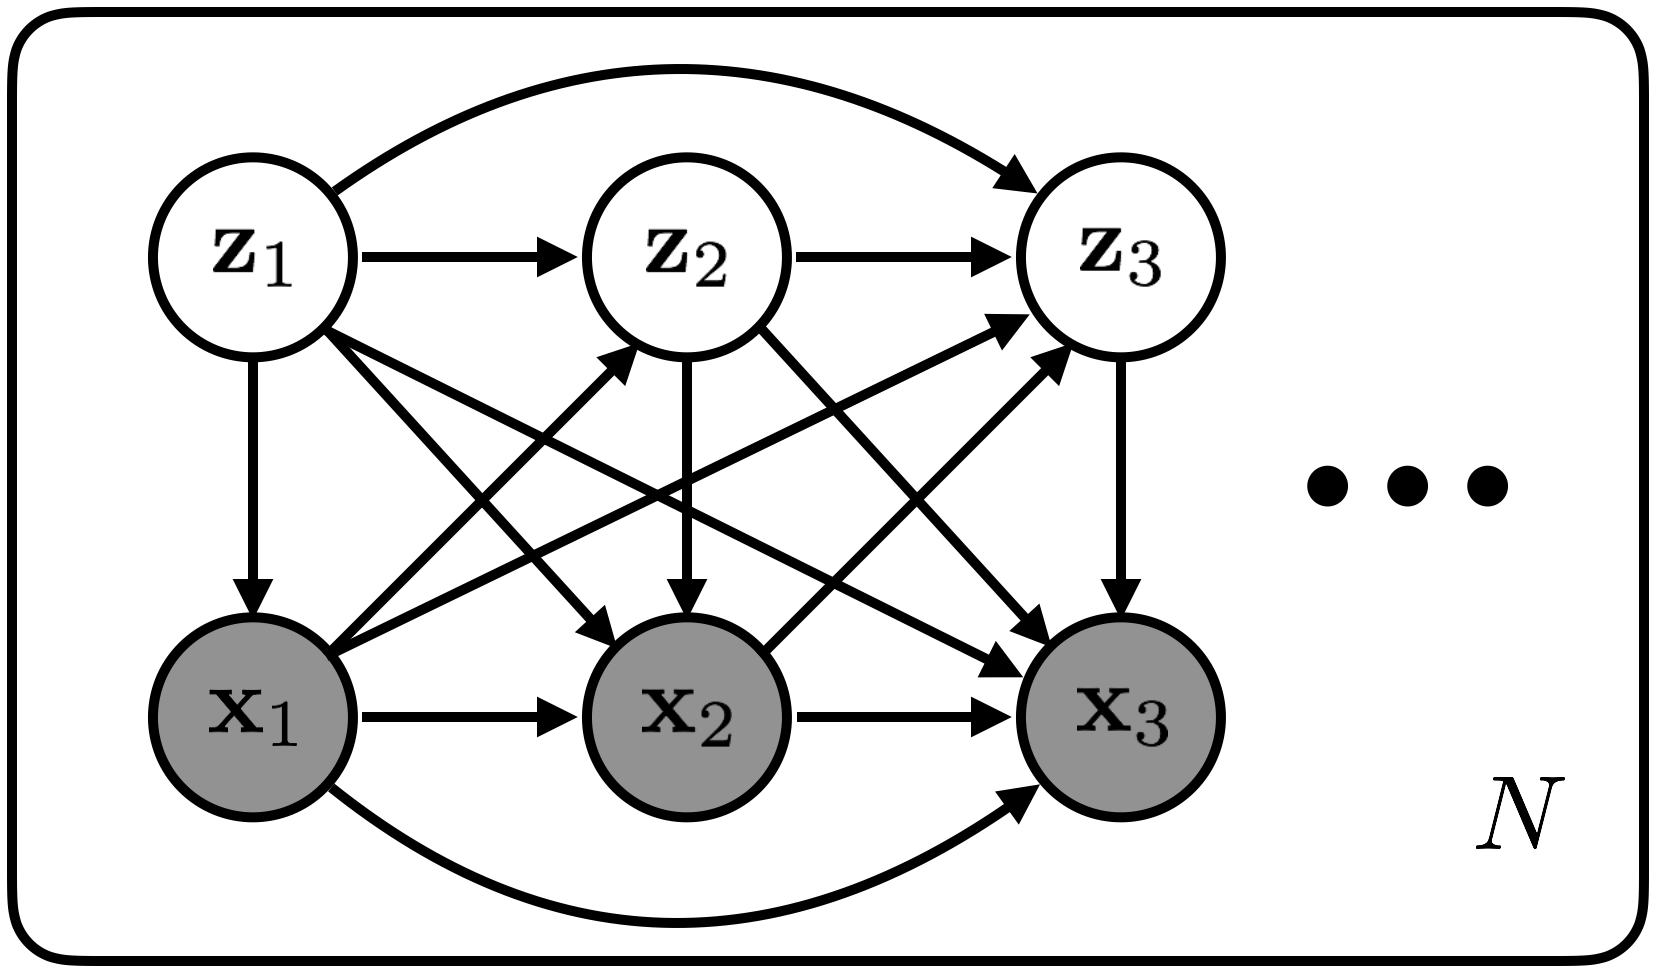
\includegraphics[width=0.8\textwidth]{images/graphical_models/full_dynamical_model.png}
        \caption{ }
        \label{fig: full_dynamical_model}
    \end{subfigure}%
    ~ 
    \begin{subfigure}[t]{0.5\textwidth}
        \centering
        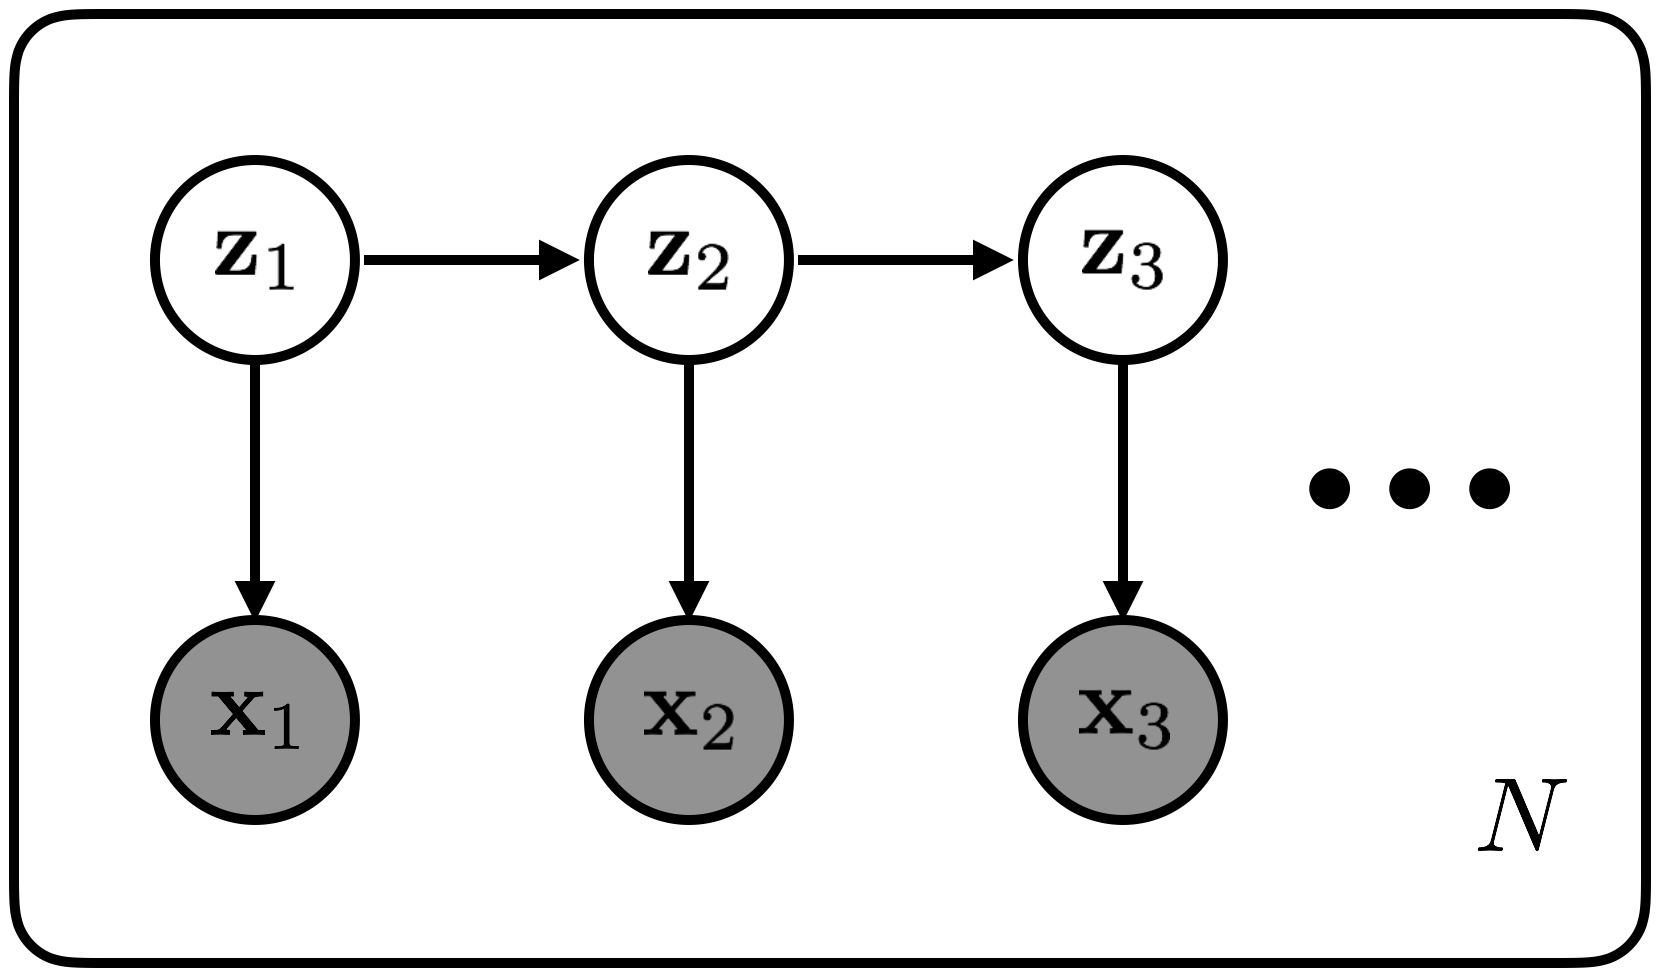
\includegraphics[width=0.8\textwidth]{images/graphical_models/markov_dynamical_model.png}
        \caption{ }
        \label{fig: markov_dynamical_model}
    \end{subfigure}
    \caption{Plate notation diagrams for dynamical latent variable models with (a) all temporal dependencies and (b) the Markov assumption. Plates denote that there are $N$ example sequences. Parameters $\theta$ have been omitted for clarity.}
\end{figure*}

\subsubsection{Bayesian Filtering}

Dynamical directed latent variable models naturally lend themselves to a \textit{filtering} setting \cite{sarkka2013bayesian}, in which one computes the marginal posterior distribution, $p(\mathbf{z}_t | \mathbf{x}_{1:t})$, at each time step. This corresponds to estimating the current state of the system given all past observations. Under the Markov assumption (eq. \ref{eq: markov dynamics model}), we start with a latent prior, $p_\theta (\mathbf{z}_1)$, and compute the marginal posterior at some time step $t$ by recursively applying the following steps:
\begin{enumerate}
	\item \textbf{Prediction}: use the Chapman-Kolmogorov equation to form a prior (i.e. prediction) on the latent variable at the next time step: 
\begin{equation}
	p(\mathbf{z}_t | \mathbf{x}_{1:t-1}) = \int p_\theta (\mathbf{z}_t | \mathbf{z}_{t-1}) p_\theta (\mathbf{z}_{t-1} | \mathbf{x}_{1:t-1}) d\mathbf{z}_{t-1}.
\end{equation}
	\item \textbf{Update}: use the prediction, along with Bayes' rule, to update the marginal posterior:
\begin{equation}
	p(\mathbf{z}_t | \mathbf{x}_{1:t}) = \frac{p_\theta (\mathbf{x}_t | \mathbf{z}_t) p_\theta (\mathbf{z}_t | \mathbf{x}_{1:t-1})}{p_\theta (\mathbf{x}_{1:t})},
\end{equation}
	where $p_\theta (\mathbf{x}_{1:t})$ is calculated as
\begin{equation}
	p_\theta (\mathbf{x}_{1:t}) = \int p_\theta (\mathbf{x}_t | \mathbf{z}_t) p_\theta (\mathbf{z}_t | \mathbf{x}_{1:t-1}) d\mathbf{z}_t.
\end{equation}
\end{enumerate}
When $p_\theta (\mathbf{x}_t | \mathbf{z}_t)$ and $p_\theta (\mathbf{z}_t | \mathbf{x}_{1:t-1})$ are parameterized as linear functions that take a Gaussian form, the resulting model is referred to as a Kalman filter \cite{kalman1961new}. However, in general, the prediction and update steps are both intractable, as they involve integrating over the space of latent variables. To overcome these intractabilities, one must turn to forms of approximate inference (see Section \ref{sec: variational inference in dynamical models}).

% The joint prior distribution of the states is given as:
% \begin{equation}
% 	p(z_{0:T}) = p(z_0) \prod_{t=1}^T p(z_t | z_{t-1}).
% \end{equation}
% The joint conditional likelihood of measurements is given as:
% \begin{equation}
% 	p(x_{1:T} | z_{0:T}) = \prod_{t=1}^T p(x_t | z_t).
% \end{equation}
% The full posterior (which is intractable) is given as:
% \begin{equation}
%	p(z_{0:T} | x_{1:T}) = \frac{p(x_{1:T} | z_{0:T}) p(z_{0:T})}{p(x_{1:T})}.
% \end{equation}

\subsubsection{Beyond the Markov Assumption}
While drastically simplifying the model, the Markov assumption is often invalid in practical settings, where one commonly encounters partial observations (i.e. hidden information) or correlated observation noise across time. In such cases, the ``memoryless" or ``static world" properties of the Markov assumption no longer hold, requiring that we expand the model to condition on past variables. This can be accomplished through
\begin{itemize}
	\item conditioning on a concatenation of variables containing the recent trajectory,
	\item memory mechanisms that selectively store state information \cite{chung2015recurrent, fraccaro2016sequential, gemici2017generative},
	\item modeling the observations and latent variables in generalized coordinates \cite{friston2010generalised}.
\end{itemize}

\section{Undirected Graphical Models}
\label{sec: undirected models}


\section{Causal Models}
\label{sec: causal models}

\subsection{Observational vs. Interventional Distributions}

This section is based on a blog post by Ferenc Husz\'ar\footnote{\texttt{http://www.inference.vc/untitled/}}. Say we have a joint probability distribution $p(x, y, z, \dots)$. Often, we are interested in conditional probabilities, for instance, how $y$ behaves given $x$. There are, in fact, two forms of this probability:
\begin{itemize}
    \item \textbf{Observational} $p(y | x)$: this is the probability of $Y = y$ given that I \textit{observe} $X = x$. This is the typical use of conditional probability in machine learning, where we simply use Bayes rule to marginalize over the joint distribution, i.e. $p(y | x) = \frac{p(y, x)}{p(x)}$.
    \item \textbf{Interventional} $p(y | do(x))$: this is the probability of $Y=y$ given that I \textit{set} $X=x$. Here, we are intervening in the data generating process. Note that the data generating process is not the same as the joint distribution.
\end{itemize}
The observational and interventional conditional probabilities are not generally the same. Ferenc gives the simple example of a sensor monitoring the value of a given quantity, such as pressure. Observing the sensor reading allows one to infer the pressure. However, intervening to change the reading on the sensor will have no effect on the pressure. Hence, $p(y|x)$ and $p(y|do(x))$ are quite different. The first simply describes statistical relationships, whereas the second describes the second describes causal relationships. The observational conditional is often sufficient for many machine learning applications, but when dealing with tasks related to decision making or control, the interventional conditional is typically more useful.

Like the observational conditional, the interventional conditional distribution, $p(y | do(x))$, is just a probability distribution that we can calculate using Bayes rule. The difference is that $p(y | do(x))$ is calculated from a separate \textit{interventional joint distribution}, $$p_{do(X=x)} (x, y, z, \dots).$$
\noindent This is the joint distribution of the variables when we conduct randomized control experiments by intervening in the data generating process to set $X=x$. Even if it is impossible or unethical to conduct these intervention experiments, this joint distribution exists. One of the main points of causal modeling is estimating the interventional conditional when we only have observations.

\begin{figure}[t!]
    \centering
    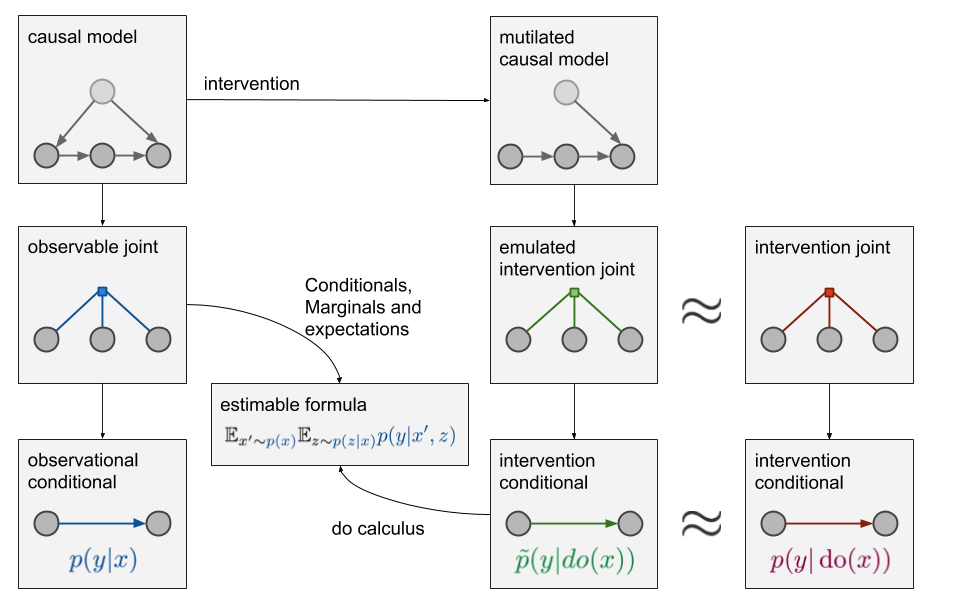
\includegraphics[width=0.8\textwidth]{images/graphical_models/Causality_-do-calculus-estimand--1-.png}
    \caption{Pipeline of causal modeling with do-calculus. Often, we only have access to the observational joint distribution, $p(x, y, z, \dots)$ but want to estimate the interventional conditional $p(y | do(x))$. To do so, we must assume a causal model and use do-calculus to arrive at an estimated interventional conditional $\tilde{p}(y | do(x))$. Note that this may not always be feasible. Reproduced from \texttt{http://www.inference.vc/untitled/}.}
    \label{fig: causal_model}
\end{figure}

\subsection{Causal Modeling \& Do-Calculus}

Supervised learning is a great technique for estimating conditional distributions. Given a joint distribution of random variables, it is fairly straightforward to train a model to estimate the conditionals. This is true of both observational and interventional conditionals, assuming one has access to the appropriate joint distribution. Recall, however, that in many cases the joint distribution contains observations rather than interventions. How, then, can we estimate the interventional conditional if we don't have direct access to the interventional joint distribution? Doing this requires making further assumptions about the structure of the data generating process. That is, we must assume a \textit{causal model} of the data, which provides information that is not captured by the observational joint distribution alone. Arrows in causal models represent direct causal directions, while the absence of an arrow denotes a lack of direct casual influence.

To estimate the interventional conditional distribution using the observational joint, one must ``mutilate" the assumed causal model to emulate the desired intervention. One then uses \textit{do-calculus} to attempt to estimate $p(y | do(x))$ from the conditionals and marginals of the observational joint distribution, yielding $\tilde{p}(y | do(x))$. Importantly, this approximation may or may not be \textit{identifiable}, depending on whether other variables in the joint distribution are observed. This pipeline is shown in Figure \ref{fig: causal_model}.


\section{Transformation of Variables}
\label{sec: transformation of variables}

Real-valued non-volume preserving (Real NVP) transformations provide a tractable method of performing learning and inference in a non-linear latent variable model \cite{dinh2016density}. With a bijective generative mapping $g$, latent variable $\mathbf{z} \sim p_z (\mathbf{z})$, and observation $\mathbf{x} \sim p_x (\mathbf{x})$, the density over observations can be modeled using the transformation of variables formula:
\begin{equation}
	p_x (\mathbf{x}) = p_z (\mathbf{z}) \bigg \vert \text{det} \left( \frac{\partial g(\mathbf{z})}{\partial \mathbf{z}^T} \right) \bigg \vert^{-1}.
	\label{eq: real nvp transform of variables 1}
\end{equation}
Using the bijection $f = g^{-1}$, equation \ref{eq: real nvp transform of variables 1} can also be written as
\begin{equation}
	p_x (\mathbf{x}) = p_z (f(\mathbf{x})) \bigg \vert \text{det} \left( \frac{\partial f(\mathbf{x})}{\partial \mathbf{x}^T} \right) \bigg \vert 
	\label{eq: real nvp transform of variables 2}
\end{equation}
\begin{equation}
	\log \left( p_x (\mathbf{x}) \right) = \log \left( p_z (f(\mathbf{x})) \right)  + \log \left( \bigg \vert \text{det} \left( \frac{\partial f(\mathbf{x})}{\partial \mathbf{x}^T} \right) \bigg \vert \right).
	\label{eq: real nvp transform of variables 3}
\end{equation}
Because the mapping between $\mathbf{x}$ and $\mathbf{z}$ is invertible, we can perform exact inference and evaluation with the model. Also note that evaluation of the log-likelihood, $\log \left( p_x (\mathbf{x}) \right)$, does not require a fixed-form reconstruction cost, such as $L^2$ distance, because the terms on the right side of eq. \ref{eq: real nvp transform of variables 3} can be computed using the data, mapping, and prior. Inference and generation procedures are shown for a simple two dimensional example in Figure \ref{fig: transform of variables}.
\begin{figure}[h]
    \centering
    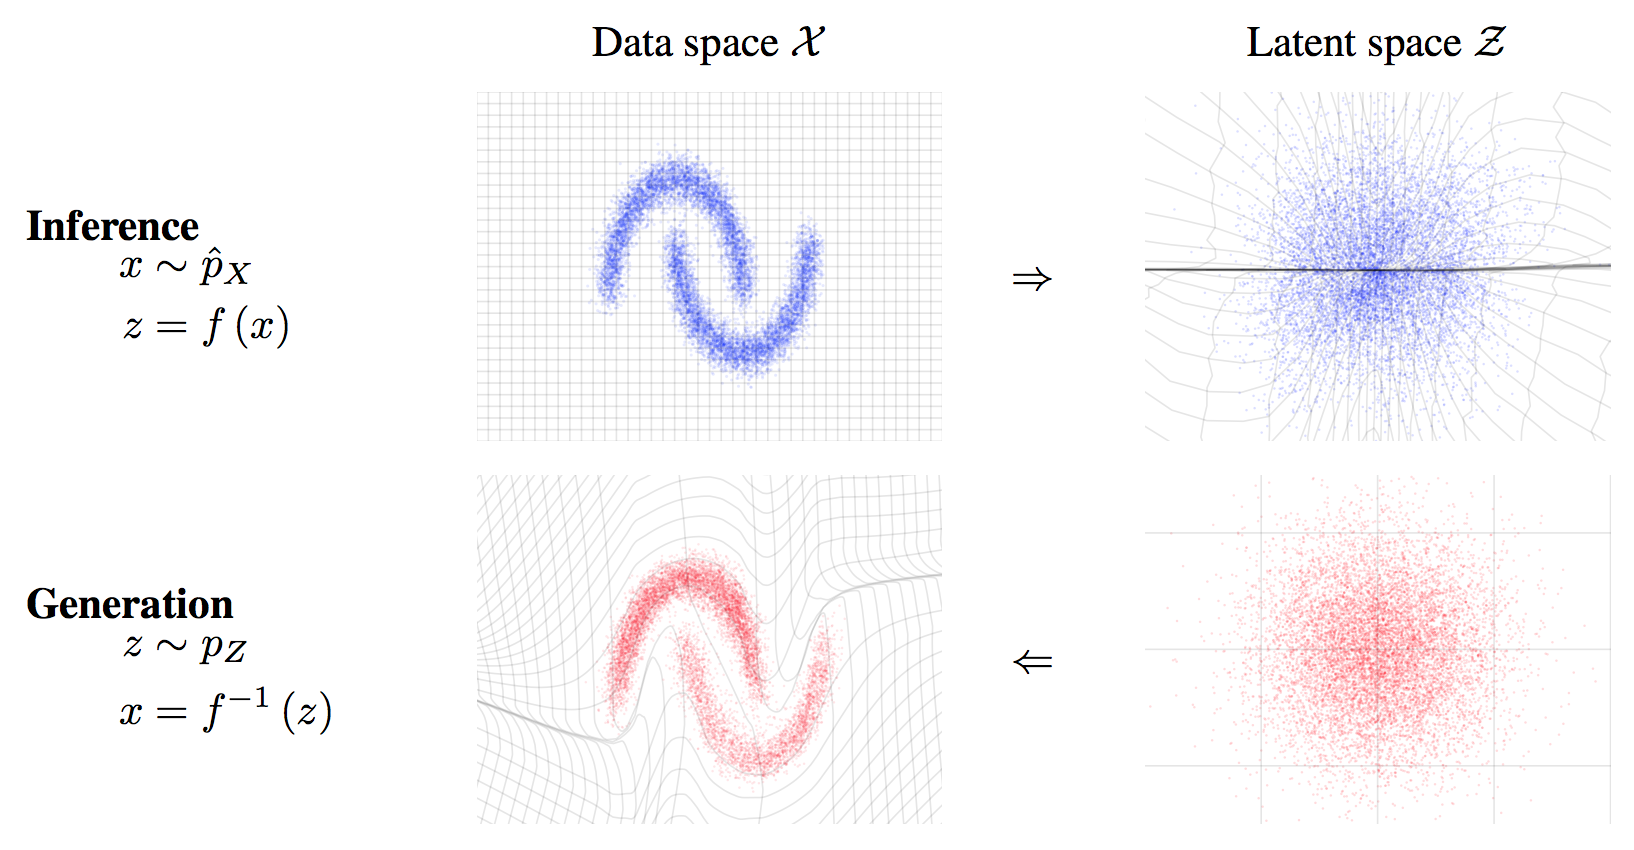
\includegraphics[width=0.8\textwidth]{images/graphical_models/transform_of_variables.png}
    \caption{Inference and generation through transformation of variables in 2D. The invertible mapping between the observed and latent variables warps the respective spaces. Reproduced from \cite{dinh2016density}.}
    \label{fig: transform of variables}
\end{figure}

In general, computing eq. \ref{eq: real nvp transform of variables 3} is intractable for high-dimensional variables, stemming from computing the log determinant of the Jacobian matrix. However, by carefully designing the mapping, we can achieve a lower triangular Jacobian matrix, the determinant of which is simply the product of the diagonal elements. Given a $D$ dimensional input $\mathbf{x}$ and $d < D$, an \textit{affine coupling layer} with output $\mathbf{y}$ is defined as 
\begin{align}
	\mathbf{y}_{1:d} &= \mathbf{x}_{1:d},
	\label{eq: real nvp mapping 1} \\
	\mathbf{y}_{d+1:D} &= \mathbf{x}_{d+1:D} \odot \exp (s(\mathbf{x}_{1:d})) + t(\mathbf{x}_{1:d}),
	\label{eq: real nvp mapping 2}
\end{align}
where $s(\mathbf{x}_{1:d})$ and $t(\mathbf{x}_{1:d})$ are respectively \textit{scale} and \textit{translation} functions from $\mathbb{R}^d \rightarrow \mathbb{R}^{D-d}$. The Jacobian of this transformation is
\begin{equation}
	\frac{\partial \mathbf{y}}{\partial \mathbf{x}^T} =
	\begin{bmatrix}
    \mathbf{I}_d & 0 \\
    \frac{\partial \mathbf{y}_{d+1:D}}{\partial \mathbf{x}^T_{1:d}}  & \text{diag} \left( \exp \left( s(\mathbf{x}_{1:d}) \right) \right)
\end{bmatrix}.
\end{equation}
Therefore, the determinant of the Jacobian can be easily computed as
\begin{equation}
	\text{det} \left( \frac{\partial \mathbf{y}}{\partial \mathbf{x}^T}  \right) = \exp \left( \sum_j s(\mathbf{x}_{1:d})_j \right).
\end{equation}
Note that $s$ and $t$ can be any arbitrary functions, as only their output values enter into inference and evaluation. Furthermore, the mapping in eqs. \ref{eq: real nvp mapping 1} and \ref{eq: real nvp mapping 2} can be inverted without computing the inverse of $s$ or $t$:
\begin{align}
	\mathbf{x}_{1:d} &= \mathbf{y}_{1:d}, \\
	\mathbf{x}_{d+1:D} &= (\mathbf{y}_{d+1:D} - t(\mathbf{x}_{1:d})) \odot \exp (- s(\mathbf{x}_{1:d})).
\end{align}
By composing multiple coupling layers, one can construct more expressive transformations. Successive coupling layers alternate between transforming different subsets of the input dimensions. The determinants of the Jacobians, as well as the inverse mappings, can still be computed easily. The authors of \cite{dinh2016density} use checkerboard and channel-wise masked convolutional networks to implement $s$ and $t$, with a hierarchy of resolutions. Other possible transformations are possible instead of coupling layers, such as normalizing and inverse auto-regressive flow.

NICE: \cite{dinh2014nice}








\chapter{Variational Inference}
\label{chap: variational inference}

\section{Inference as Optimization: Deriving the ELBO}

Consider a model, $p(\mathbf{x}, \mathbf{z})$, that specifies a joint distribution over a latent variable $\mathbf{z}$ and observed variable $\mathbf{x}$. To infer the posterior distribution of $\mathbf{z}$ given $\mathbf{x}$, we can use the definition of conditional probability:

\begin{equation}
	p (\mathbf{z} | \mathbf{x}) = \frac{p(\mathbf{x}, \mathbf{z})}{p (\mathbf{x})},
	\label{eq: bayes rule}
\end{equation}

\noindent where the marginal likelihood (a.k.a. model evidence or partition function) $p(\mathbf{x})$ is calculated by marginalizing over the latent state space:

\begin{equation}
	p (\mathbf{x}) = \int p(\mathbf{x}, \mathbf{z}) d\mathbf{z}.
	\label{eq: marginalize}
\end{equation}

 \noindent For large latent spaces and/or complicated models, performing the integration in eq. \ref{eq: marginalize} is computationally intractable.
 
 Variational inference transforms this intractable integration problem into an \textit{optimization} problem by introducing an approximate posterior distribution, $q (\mathbf{z} | \mathbf{x})$, typically chosen from some simple family of distributions, such as independent Gaussians. We attempt to make $q (\mathbf{z} | \mathbf{x})$ as ``close" as possible to $p (\mathbf{z} | \mathbf{x})$ by minimizing $ D_{KL}(q (\mathbf{z} | \mathbf{x}) || p (\mathbf{z} | \mathbf{x}))$. Notice that the word close is in quotations because KL divergence is not a true distance measure; it is not symmetric. When the (non-negative) KL divergence between these distributions is zero, we recover the true posterior, $p (\mathbf{z} | \mathbf{x})$. We cannot evaluate $ D_{KL}(q (\mathbf{z} | \mathbf{x}) || p (\mathbf{z} | \mathbf{x}))$ directly, as it includes the true posterior, which we cannot tractably compute. Instead, we will maximize a lower bound on $p(\mathbf{x})$, which will have the effect of minimizing $ D_{KL}(q (\mathbf{z} | \mathbf{x}) || p (\mathbf{z} | \mathbf{x}))$, which we will now show. We start from the definition of KL divergence:
 
 \begin{equation}
 	D_{KL}(q (\mathbf{z} | \mathbf{x}) || p (\mathbf{z} | \mathbf{x})) = \mathbb{E}_{\mathbf{z} \sim q (\mathbf{z} | \mathbf{x})} \left[ \log \frac{q (\mathbf{z} | \mathbf{x})}{p (\mathbf{z} | \mathbf{x})} \right],
	\label{eq: elbo derivation 1}
 \end{equation}
 
 
 \begin{equation}
 	D_{KL}(q (\mathbf{z} | \mathbf{x}) || p (\mathbf{z} | \mathbf{x})) = \mathbb{E}_{\mathbf{z} \sim q (\mathbf{z} | \mathbf{x})} \left[ \log q (\mathbf{z} | \mathbf{x}) \right] - \mathbb{E}_{\mathbf{z} \sim q (\mathbf{z} | \mathbf{x})} \left[ \log p (\mathbf{z} | \mathbf{x}) \right].
	\label{eq: elbo derivation 2}
 \end{equation}
 
 \noindent Plugging in the definition of conditional probability into the second term yields:
 
  \begin{equation}
 	D_{KL}(q (\mathbf{z} | \mathbf{x}) || p (\mathbf{z} | \mathbf{x})) = \mathbb{E}_{\mathbf{z} \sim q (\mathbf{z} | \mathbf{x})} \left[ \log q (\mathbf{z} | \mathbf{x}) \right] - \mathbb{E}_{\mathbf{z} \sim q (\mathbf{z} | \mathbf{x})} \left[ \log \frac{p (\mathbf{x}, \mathbf{z})}{p (\mathbf{x})} \right],
	\label{eq: elbo derivation 3}
 \end{equation}
 
 \noindent which can be expanded into
 \begin{equation}
 	D_{KL}(q (\mathbf{z} | \mathbf{x}) || p (\mathbf{z} | \mathbf{x})) = \mathbb{E}_{\mathbf{z} \sim q (\mathbf{z} | \mathbf{x})} \left[ \log q (\mathbf{z} | \mathbf{x}) \right] - \mathbb{E}_{\mathbf{z} \sim q (\mathbf{z} | \mathbf{x})} \left[ \log p (\mathbf{x}, \mathbf{z}) \right] + \log p (\mathbf{x}).
	\label{eq: elbo derivation 4}
 \end{equation}
 
 \noindent Now, we'll define the following quantity, which we refer to as the \textit{evidence lower bound (ELBO)} or \textit{variational lower bound} or \textit{negative free energy}:
 
\begin{equation}
 	\boxed{\mathcal{L} \equiv \mathbb{E}_{\mathbf{z} \sim q (\mathbf{z} | \mathbf{x})} \left[ \log p (\mathbf{x}, \mathbf{z}) - \log q (\mathbf{z} | \mathbf{x}) \right]}
	\label{eq: elbo derivation 5}
\end{equation}

\noindent Plugging this definition back into eq. \ref{eq: elbo derivation 4}, we get

   \begin{equation}
 	D_{KL}(q (\mathbf{z} | \mathbf{x}) || p (\mathbf{z} | \mathbf{x})) = \log p (\mathbf{x})  - \mathcal{L}.
	\label{eq: elbo derivation 6}
 \end{equation}
 
 \noindent Rearranging terms, we see
 
    \begin{equation}
 	\log p (\mathbf{x})  =  \mathcal{L} + D_{KL}(q (\mathbf{z} | \mathbf{x}) || p (\mathbf{z} | \mathbf{x})).
	\label{eq: elbo derivation 7}
 \end{equation}

\noindent Since $D_{KL}(q (\mathbf{z} | \mathbf{x}) || p (\mathbf{z} | \mathbf{x}))$ is non-negative, $\mathcal{L}$ is a lower bound on $\log p (\mathbf{x})$. Further, since $\log p (\mathbf{x})$ is not dependent on $q (\mathbf{z} | \mathbf{x})$, we see that maximizing $\mathcal{L}$ with respect to $q (\mathbf{z} | \mathbf{x})$ must minimize $D_{KL}(q (\mathbf{z} | \mathbf{x}) || p (\mathbf{z} | \mathbf{x}))$. Thus, we can approximate the true posterior by optimizing $\mathcal{L}$ with respect to $q (\mathbf{z} | \mathbf{x})$.

Note that the ELBO can also be written in the following form:

\begin{equation}
 	\mathcal{L} = \mathbb{E}_{\mathbf{z} \sim q (\mathbf{z} | \mathbf{x})} \left[ \log p (\mathbf{x}, \mathbf{z}) - \log q (\mathbf{z} | \mathbf{x}) \right]
	\label{eq: elbo derivation 8}
 \end{equation}
 
\begin{equation}
 	\mathcal{L} = \mathbb{E}_{\mathbf{z} \sim q (\mathbf{z} | \mathbf{x})} \left[ \log p (\mathbf{x} | \mathbf{z})  + \log p(\mathbf{z}) - \log q (\mathbf{z} | \mathbf{x}) \right]
	\label{eq: elbo derivation 9}
 \end{equation}
 
\begin{equation}
 	\mathcal{L} = \mathbb{E}_{\mathbf{z} \sim q (\mathbf{z} | \mathbf{x})} \left[ \log p (\mathbf{x} | \mathbf{z}) \right] - D_{KL}(q (\mathbf{z} | \mathbf{x}) || p (\mathbf{z}))
	\label{eq: elbo derivation 10}
 \end{equation}

\noindent This highlights that the ELBO specifies the optimal $q (\mathbf{z} | \mathbf{x})$ by trading off between representing the input, through the first term, and agreeing with the prior on the latent variables, through the second term. In other words, the first term attempts to fit the data, while the second term regularizes the representation.



\section{Normalizing Flows} 

A common drawback of variational inference is that it is typically restricted to families of approximate posterior densities, e.g. factorized Gaussians. \textit{Normalizing flows} \cite{rezende2015variational} is a method for fitting flexible approximate posterior densities. It uses a sequence of invertible mappings, called a `flow,' to transform simple posterior densities into arbitrary, flexible forms. If we start with a variable $\mathbf{z}$, drawn from a distribution $q(\mathbf{z})$, and apply an invertible, smooth mapping $f(\mathbf{z})$, then the change of variables formula allows us to write

\begin{equation}
q(\mathbf{z}^\prime) = q(\mathbf{z}) \text{det} \bigg\vert \frac{\partial f^{-1}}{\partial \mathbf{z}^\prime} \bigg\vert = q(\mathbf{z}) \text{det} \bigg\vert \frac{\partial f}{\partial \mathbf{z}} \bigg\vert^{-1}.
\end{equation}
\newline

\begin{figure}[h]
    \centering
    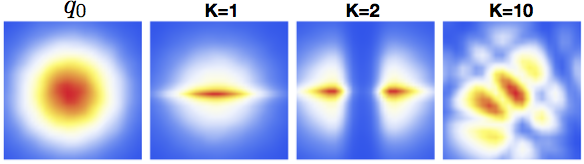
\includegraphics[width=.6\textwidth]{images/graphical_models/normalizing_flows.png}
    \caption{Normalizing flows applied to a 2D isotropic Gaussian, using transformations of the form given in eq. \ref{eq: normalizing flows transformation}. Increasing the flow length $K$ allows for more flexible approximate posterior distributions. Reproduced from \cite{rezende2015variational}.}
    \label{fig: normalizing flows}
\end{figure}

\noindent Note that the mapping, $f$, can also depend on other inputs, such as observed variables $\mathbf{x}$ or other auxiliary inputs. By composing multiple mappings, we can construct arbitrarily complex densities. Thus, starting from an initial distribution of $q_0 (\mathbf{z}_0)$, a flow of length $K$ can be computed as

\begin{equation}
	\log q_K (\mathbf{z}_K) = \log q_0 (\mathbf{z}_0) - \sum_{k=1}^K \log \text{det}  \bigg\vert \frac{\partial f_k}{\partial \mathbf{z}_{k-1}} \bigg\vert.
\end{equation}

\noindent This sequence can be interpreted as performing expansions and contractions on the initial density to construct a more flexible form. 

To parameterize the mappings, \cite{rezende2015variational} use transformations of the form

\begin{equation}
	f(\mathbf{z}) = \mathbf{z} + \mathbf{u}h(\mathbf{w}^\intercal \mathbf{z} + b)
	\label{eq: normalizing flows transformation}
\end{equation}

\noindent where $\mathbf{u}$, $\mathbf{w}$, and $b$ are learned parameters and $h(\cdot)$ is a non-linear function. This class of normalizing flows is referred to as $planar flows$. The determinant of the Jacobian of this transformation is

\begin{equation}
	\text{det} \bigg\vert  \frac{\partial f}{\partial \mathbf{z}} \bigg\vert = \big\vert \text{det} \left( \mathbf{I} + \mathbf{u} (h^\prime (\mathbf{w}^\intercal \mathbf{z} + b) \mathbf{w})^\intercal \right) \big\vert = \big\vert 1 + \mathbf{u}^\intercal h^\prime (\mathbf{w}^\intercal \mathbf{z} + b) \mathbf{w} \big\vert
\end{equation}

\noindent Finally, putting everything together, we can use normalizing flows to draw samples from the final, more flexible approximate posterior, $q(\mathbf{z} | \mathbf{x}) = q_K (\mathbf{z}_K)$. The variational lower bound becomes

\begin{equation}
	\mathcal{L} = \mathbb{E}_{\mathbf{z} \sim q(\mathbf{z}, \mathbf{x})} \left[ \log p(\mathbf{x}, \mathbf{z}) - \log q(\mathbf{z}|\mathbf{x}) \right]
	\label{eq: norm flows lower bound 1}
\end{equation}

\begin{equation}
	\mathcal{L} = \mathbb{E}_{\mathbf{z}_0 \sim q(\mathbf{z}_0, \mathbf{x})} \left[ \log p(\mathbf{x}, \mathbf{z}_K) - \log q(\mathbf{z}_0|\mathbf{x}) + \sum_{k=1}^K \log \big\vert 1 + \mathbf{u}_k^\intercal h_k^\prime (\mathbf{w}_k^\intercal \mathbf{z}_{k-1} + b_k) \mathbf{w}_k \big\vert \right]
	\label{eq: norm flows lower bound 2}
\end{equation}

\noindent Note that in going to eq. \ref{eq: norm flows lower bound 1} to eq. \ref{eq: norm flows lower bound 2} we have used the \textit{law of the unconscious statistician (LOTUS)}, which allows one to take expectations of a transformed variable (or any function thereof) using the original variable. If $\mathbf{z}^\prime = f(\mathbf{z})$ and $g$ is some arbitrary function of $\mathbf{z}^\prime$, then this can be expressed as

\begin{equation}
	\mathbb{E}_{\mathbf{z}^\prime \sim q (\mathbf{z}^\prime)} \left[ g(\mathbf{z}^\prime) \right] = \mathbb{E}_{\mathbf{z} \sim q (\mathbf{z})} \left[ g( f (\mathbf{z})) \right].
\end{equation}

\noindent Thus, we can take expectations with respect to the final density, i.e. the approximate posterior, using samples drawn from the initial density. In an amortized inference setting, the inference model can output the parameters of the initial distribution as well as parameters for each stage of the flow. The flow parameters could also be learned as global parameters.


Another class of normalizing flows is \textit{inverse auto-regressive flow (IAF)} \cite{kingma2016improved}. These transformations take inspiration from auto-regressive models, which factor joint probability distributions into a series of conditional distributions using the chain rule of probability.


\section{Filtering Variational Inference}
\label{sec: variational inference in dynamical models}

We assume the dynamic directed latent variable model set-up given in Section \ref{sec: dynamical latent variable models}. We can bound the marginal log-likelihood of the observation sequence by introducing an approximate posterior distribution, $q(\mathbf{z}_{1:T} | \mathbf{x}_{1:T})$, then using Jensen's inequality to write
\begin{equation}
    \log p(\mathbf{x}_{1:T}) \geq \mathbb{E}_{q(\mathbf{z}_{1:T} | \mathbf{x}_{1:T})} \left[ \log \frac{p(\mathbf{x}_{1:T} , \mathbf{z}_{1:T})}{q(\mathbf{z}_{1:T} | \mathbf{x}_{1:T})} \right] \equiv - \mathcal{F}_E,
    \label{eq: vi_1}
\end{equation}
where $\mathcal{F}_E$ is the total \textit{variational free-energy}. For now, we assume the generative model takes the form given by eq. \ref{eq: general dynamics model}, and the approximate posterior takes the form:
\begin{equation}
    q(\mathbf{z}_{1:T} | \mathbf{x}_{1:T}) = \prod_{t=1}^T q(\mathbf{z}_t | \mathbf{x}_{1:t} , \mathbf{z}_{1:t-1}).
    \label{eq: approx post form}
\end{equation}
In other words, we assume we are in the online setting, and therefore use a \textit{filtering} approximate posterior that does not condition on future observations or latent variables. Using eqs. \ref{eq: general dynamics model} and \ref{eq: approx post form}, we can rewrite eq. \ref{eq: vi_1} as
\begin{equation}
    \log p(\mathbf{x}_{1:T}) \geq \mathbb{E}_{q(\mathbf{z}_{1:T} | \mathbf{x}_{1:T})} \left[ \sum_{t=1}^T \log \frac{p(\mathbf{x}_t | \mathbf{x}_{1:t-1} , \mathbf{z}_{1:t}) p(\mathbf{z}_t | \mathbf{x}_{1:t-1} , \mathbf{z}_{1:t-1})}{q(\mathbf{z}_t | \mathbf{x}_{1:t} , \mathbf{z}_{1:t-1})} \right].
\end{equation}
Defining the term
\begin{equation}
    C_t \equiv \log \frac{p(\mathbf{x}_t | \mathbf{x}_{1:t-1} , \mathbf{z}_{1:t}) p(\mathbf{z}_t | \mathbf{x}_{1:t-1} , \mathbf{z}_{1:t-1})}{q(\mathbf{z}_t | \mathbf{x}_{1:t} , \mathbf{z}_{1:t-1})},
\end{equation}
then
\begin{align}
    \log p(\mathbf{x}_{1:T}) & \geq \mathbb{E}_{q(\mathbf{z}_{1:T} | \mathbf{x}_{1:T})} \left[ \sum_{t=1}^T C_t \right] \\
    & = \mathbb{E}_{q(\mathbf{z}_1 | \mathbf{x}_1)} \mathbb{E}_{q(\mathbf{z}_2 | \mathbf{x}_{1:2} , \mathbf{z}_1)} \dots \mathbb{E}_{q(\mathbf{z}_T | \mathbf{x}_{1:T} , \mathbf{z}_{1:T-1})} \left[ \sum_{t=1}^T C_t \right].
\end{align}
% \begin{align}
%     \log p(\mathbf{x}_{1:T}) & \geq \mathbb{E}_{q(\mathbf{z}_{1:T} | \mathbf{x}_{1:T})} \left[ \sum_{t=1}^T C_t \right] \\
%     & = \int_{\mathbf{z}_1} q(\mathbf{z}_1 | \mathbf{x}_1) \int_{\mathbf{z}_2} q(\mathbf{z}_2 | \mathbf{z}_1 , \mathbf{x}_{1:2}) \int_{\mathbf{z}_3} \dots \int_{\mathbf{z}_T} q(\mathbf{z}_T | \mathbf{z}_{1:T-1} , \mathbf{x}_{1:T}) \sum_{t=1}^T C_t
% \end{align}
There are $T$ terms within the sum, but because we do not condition on future variables, each $C_t$ only depends on the expectations up to time $t$. This allows us to write:
\begin{align}
    \log p(\mathbf{x}_{1:T}) & \geq \mathbb{E}_{q(\mathbf{z}_1 | \mathbf{x}_1)} \left[ C_1 \right] \nonumber \\ 
    & + \mathbb{E}_{q(\mathbf{z}_1 | \mathbf{x}_1)} \mathbb{E}_{q(\mathbf{z}_2 | \mathbf{z}_1 , \mathbf{x}_{1:2})} \left[ C_2 \right] \nonumber \\
    & + \dots \nonumber \\
    & + \mathbb{E}_{q(\mathbf{z}_1 | \mathbf{x}_1)} \mathbb{E}_{q(\mathbf{z}_2 | \mathbf{z}_1 , \mathbf{x}_{1:2})} \dots \mathbb{E}_{q(\mathbf{z}_T | \mathbf{z}_{1:T-1} , \mathbf{x}_{1:T})} \left[ C_T \right] \\
    & = \sum_{t=1}^T \mathbb{E}_{q(\mathbf{z}_{1:t} | \mathbf{x}_{1:t})} \left[ C_t \right] \\
    & = \sum_{t=1}^T \mathbb{E}_{\prod_{\tau=1}^t q(\mathbf{z}_\tau | \mathbf{x}_{1:\tau} , \mathbf{z}_{1:\tau-1})} \left[ C_t \right] \\
    & = \sum_{t=1}^T \mathbb{E}_{\prod_{\tau=1}^{t-1} q(\mathbf{z}_\tau | \mathbf{x}_{1:\tau} , \mathbf{z}_{1:\tau-1})} \left[ \mathbb{E}_{q(\mathbf{z}_t | \mathbf{x}_{1:t} , \mathbf{z}_{1:t-1})} \left[ C_t \right] \right]
\end{align}
% \begin{align}
%     \log p(\mathbf{x}_{1:T}) & \geq \int_{\mathbf{z}_1} q(\mathbf{z}_1 | \mathbf{x}_1) C_1 \\ 
%     & + \int_{\mathbf{z}_1} q(\mathbf{z}_1 | \mathbf{x}_1) \int_{\mathbf{z}_2} q(\mathbf{z}_2 | \mathbf{z}_1 , \mathbf{x}_{1:2}) C_2 \\
%     & + \dots \\
%     & + \int_{\mathbf{z}_1} q(\mathbf{z}_1 | \mathbf{x}_1) \int_{\mathbf{z}_2} q(\mathbf{z}_2 | \mathbf{z}_1 , \mathbf{x}_{1:2}) \dots \int_{\mathbf{z}_T} q(\mathbf{z}_T | \mathbf{z}_{1:T-1} , \mathbf{x}_{1:T}) C_T \\
%     & = \sum_{t=1}^T \mathbb{E}_{q(\mathbf{z}_{1:t} | \mathbf{x}_{1:t})} \left[ C_t \right] \\
%     & = \sum_{t=1}^T \mathbb{E}_{\prod_{\tau=1}^t q(\mathbf{z}_\tau | \mathbf{x}_{1:\tau} , \mathbf{z}_{1:\tau-1})} \left[ C_t \right] \\
%     & = \sum_{t=1}^T \mathbb{E}_{\prod_{\tau=1}^{t-1} q(\mathbf{z}_\tau | \mathbf{x}_{1:\tau} , \mathbf{z}_{1:\tau-1})} \left[ \mathbb{E}_{q(\mathbf{z}_t | \mathbf{x}_{1:t} , \mathbf{x}_{1:t})} \left[ C_t \right] \right] \\
% \end{align}
The total variational free-energy is thus the sum of per-time-step variational free-energies, with expectations taken w.r.t. all past latent variables:
\begin{equation}
    \mathcal{F}_E = - \sum_{t=1}^T \mathbb{E}_{\prod_{\tau=1}^{t-1} q(\mathbf{z}_\tau | \mathbf{x}_{1:\tau} , \mathbf{z}_{1:\tau-1})} \left[ \mathbb{E}_{q(\mathbf{z}_t | \mathbf{x}_{1:t} , \mathbf{z}_{1:t-1})} \left[ C_t \right] \right].
\end{equation}

Evaluating these outer expectations becomes computationally intractable as the sequence length grows. When approximating each of the $T$ expectations with $m$ Monte Carlo samples, evaluating the summation requires drawing $\mathcal{O}(m^T)$ samples. For $m > 1$, the number of samples, and therefore the amount of computation, blows up as $T \rightarrow \infty$. Thus, to retain tractability, we can set $m=1$ for expectations over all past time steps, thereby evaluating the path summation of the per time step variational free-energies, defined as the \textit{variational free-action}, $\mathcal{F}_A$:
\begin{equation}
    \mathcal{F}_A \equiv - \sum_{t=1}^T \mathbb{E}_{q(\mathbf{z}_t | \mathbf{x}_{1:t} , \mathbf{z}_{1:t-1})} \left[ C_t \right] \bigg \vert_{\mathbf{z}_{1:t-1}}
\end{equation}
where $\mathbf{z}_{1:t-1}$ is the sampled trajectory of the past latent variables. The free-action evaluates a single path through the latent space, whereas the free-energy evaluates all possible paths. However, the free-action still provides a lower bound on the marginal log-likelihood of the sequence. Need to show this...

\chapter{Mathematical Tools \& Tricks}
\label{chap: math tools and tricks}

\section{Differentiation}
\label{sec: differentiation}

Differentiation is \textit{the} core mathematical operation required for gradient-based optimization, which arises in both learning and inference procedures. However, standard differentiation tools are not adequate for handling functions containing non-differentiable elements, such as discontinuities and/or stochastic computations. In these cases, we can rely on a variety of techniques to \textit{estimate} derivatives. Some recent work in differentiation: Gumbel-Softmax \cite{jang2016categorical}, Concrete \cite{maddison2016concrete}, REBAR \cite{tucker2017rebar}, RELAX \cite{grathwohl2017backpropagation}. See also \cite{schulman2015gradient} for an overview of gradient estimation in stochastic computation graphs.

\subsection{Score Function Estimator}
\label{subsec: score function estimator}

[From Shakir Mohamed's \href{http://blog.shakirm.com/2015/11/machine-learning-trick-of-the-day-5-log-derivative-trick/}{blog}.] The score function estimator (also called REINFORCE \cite{williams1992simple}) can be used to estimate gradients of the following form:
\begin{equation}
    \nabla_\theta \mathbb{E}_{p(\mathbf{z}; \theta)} \left[ f(\mathbf{z}) \right],
    \nonumber
\end{equation}
in which $\theta$ are the parameters of a parametric distribution, $p(\mathbf{z}; \theta)$. Often, we estimate the expectation through sampling $\mathbf{z} \sim p(\mathbf{z}; \theta)$, which is non-differentiable w.r.t $\theta$. Gradients of this form occur, for instance, in variational inference (Chapter \ref{chap: variational inference}), where $\theta$ are the parameters of the approximate posterior, and policy gradient methods in reinforcement learning (Section \ref{sec: policy search methods}), where $\theta$ are the parameters of the policy. To estimate this gradient, the score function estimator employs the \textbf{log-derivative trick}:
\begin{equation}
    \nabla_\theta \log p(\mathbf{z}; \theta) = \frac{\nabla_\theta p(\mathbf{z}; \theta)}{p(\mathbf{z}; \theta)}.
\end{equation}
The expression $\nabla_\theta \log p(\mathbf{z}; \theta)$ is referred to as the \textit{score function}, and the expression on the right is referred to as the \textit{score ratio}. Note that the expected value of the score function is zero:
\begin{equation}
\begin{split}
    \mathbb{E}_{p(\mathbf{z}; \theta)} \left[ \nabla_\theta \log p(\mathbf{z}; \theta) \right] & = \mathbb{E}_{p(\mathbf{z}; \theta)} \left[ \frac{\nabla_\theta p(\mathbf{z}; \theta)}{p(\mathbf{z}; \theta)} \right] \\
    & = \int p(\mathbf{z}; \theta) \frac{\nabla_\theta p(\mathbf{z}; \theta)}{p(\mathbf{z}; \theta)} d \mathbf{z} \\
    & = \nabla_\theta \int p(\mathbf{z}; \theta) d \mathbf{z} \\
    & = \nabla_\theta 1 = 0.
\end{split}
\end{equation}
In the third line, we have exchanged differentiation and integration, which we assume is valid. The fact that the expected value is zero allows us to subtract any terms from the score function that have zero expectation while leaving the expected score unaffected. This technique is referred to as control variates (see below). The variance of the score function is the Fisher information:
\begin{equation}
    \mathbb{V} \left[ \nabla_\theta \log p(\mathbf{z}; \theta) \right] = \mathcal{I} (\theta) \equiv \mathbb{E}_{p(\mathbf{z}; \theta)} \left[ \nabla_\theta \log p(\mathbf{z}; \theta) \nabla_\theta \log p(\mathbf{z}; \theta)^\intercal \right].
\end{equation}
Now, we can use the log-derivative trick to estimate the gradient from the original expression.
\begin{equation}
\begin{split}
    \nabla_\theta \mathbb{E}_{p(\mathbf{z}; \theta)} \left[ f(\mathbf{z}) \right] & = \nabla_\theta \int p(\mathbf{z}; \theta) f(\mathbf{z}) d \mathbf{z} \\
    & = \int \nabla_\theta p(\mathbf{z}; \theta) f(\mathbf{z}) d \mathbf{z} \\
    & = \int \frac{p(\mathbf{z}; \theta)}{p(\mathbf{z}; \theta)} \nabla_\theta p(\mathbf{z}; \theta) f(\mathbf{z}) d \mathbf{z} \\
    & = \int p(\mathbf{z}; \theta) \nabla_\theta \log p(\mathbf{z}; \theta) f(\mathbf{z}) d \mathbf{z} \\
    & = \mathbb{E}_{p(\mathbf{z}; \theta)} \left[ f(\mathbf{z}) \nabla_\theta \log p(\mathbf{z}; \theta) \right] \\
    & \approx \frac{1}{S} \sum_{s=1}^S f(\mathbf{z}^{(s)}) \nabla_\theta \log p(\mathbf{z}^{(s)}; \theta),
\end{split}
\end{equation}
where, in the last line, $\mathbf{z}^{(s)} \sim p(\mathbf{z}; \theta)$. The log-derivative trick was used in transitioning from the third to the fourth line. Note that $f(\mathbf{z})$ does not need to be differentiable. That is, as long as we can evaluate $f(\mathbf{z})$ for a given value of $\mathbf{z}$, we can effectively treat it as a black box (see, e.g. black box variational inference (BBVI) \cite{ranganath2014black}). This is a useful quality, as it allows us to estimate gradients using, for example, reward functions in reinforcement learning. The score function estimator allows us to change a gradient of an expectation into an expectation of a gradient. This estimator is unbiased, but tends to suffer from high variance. To reduce the variance, we can use a \textit{control variate}, $\lambda$, a function with zero mean:
\begin{equation}
    \nabla_\theta \mathbb{E}_{p(\mathbf{z}; \theta)} \left[ f(\mathbf{z}) \right] =  \mathbb{E}_{p(\mathbf{z}; \theta)} \left[ \left( f(\mathbf{z}) - \lambda \right) \nabla_\theta \log p(\mathbf{z}; \theta) \right].
\end{equation}
In reinforcement learning, control variates are commonly referred to as \textit{baselines}.


\subsection{Pathwise Derivative Estimator}

With the score function estimator (Section \ref{subsec: score function estimator}), we saw that we could estimate the gradient of an expectation of some function w.r.t. the parameters of the expectation distribution. We could effectively treat the function within the expectation as a black box, however, the resulting gradient estimator suffered from high variance. In other cases, we may have direct access to the function $f(\mathbf{z})$, and we may be able to reparameterize the sampling procedure in terms of simpler distributions, which do not depend on the parameters, $\theta$. In such cases, we can employ the pathwise derivative estimator, also known as the \textit{reparameterization trick} \cite{rezende2014stochastic, kingma2013auto}.


\part{Neuroscience}
\chapter{Anatomy \& Function}
\label{chap: anatomy}

\section{Introduction}

The mammalian central nervous system is often divided into the brain stem, limbic system, cerebellum, and cerebrum. The brain stem, which sits at the base, is composed of the medulla, pons, and mid-brain. It plays a role in regulating basic biological functions, such as heart rate, breathing, eating, sleeping, etc. The limbic system is a collection of structures that sit on top of the brain stem. These structures consist of the hippocampal formation, hypothalamus, thalamus, and amygdala. The cerebellum sits behind the other areas, and is a dense, highly folded sheet of neurons that is often associated with posture and movement. The cerebrum contains the cerebral cortex, another highly folded sheet of neurons, consisting of four lobes that sit on top of the limbic system. It is associated with a variety of ``higher order" cognitive capacities, such as sensory processing, memory, language, movement, planning, etc. The cerebrum also contains a variety of sub-cortical structures, such as the basal ganglia and olfactory bulb.


\section{Brain Stem}

\subsection{Midbrain}

\subsection{Pons}

\subsection{Medulla Oblongata}


\section{Limbic System}

Limbic system is shown in Figure \ref{fig: limbic system}.

\begin{figure}[h]
    \centering
    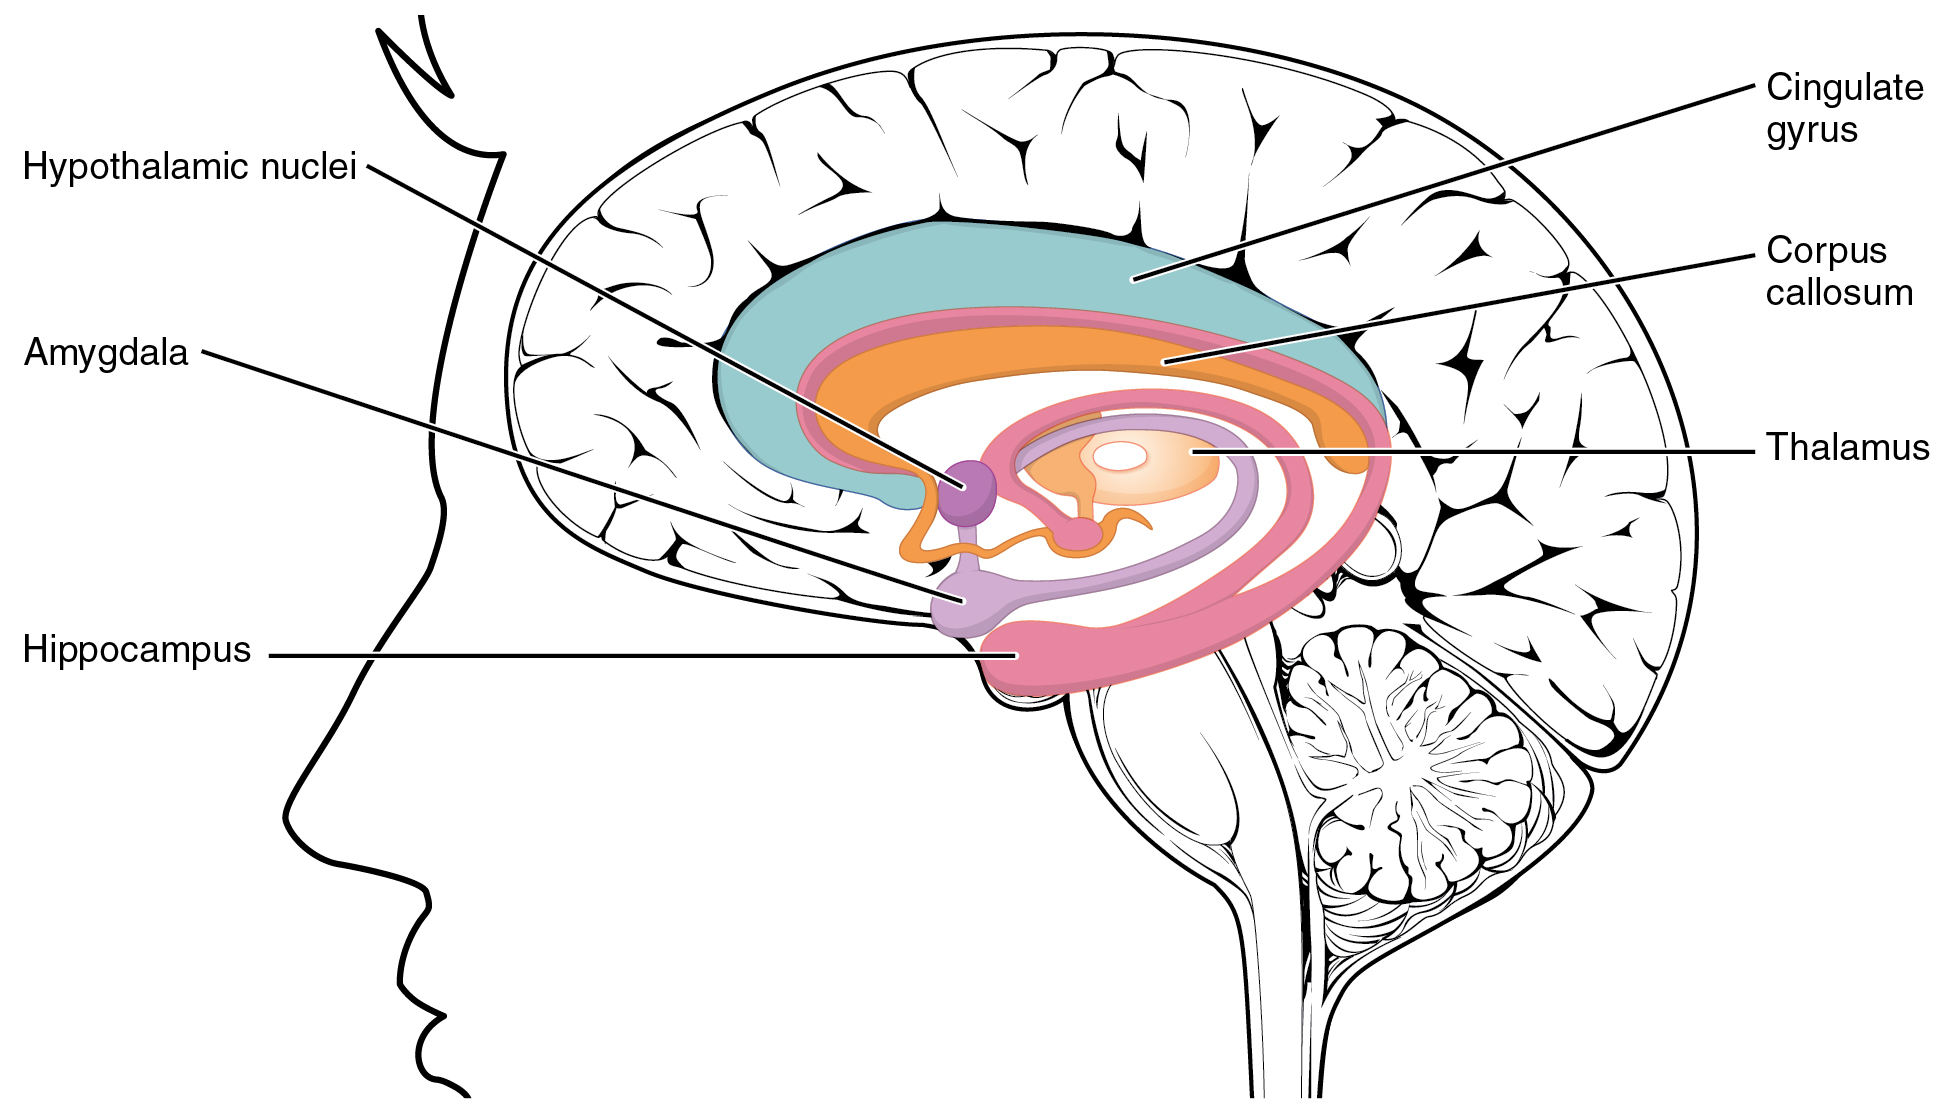
\includegraphics[width=.75\textwidth]{images/neuroscience/limbic_system.jpg}
    \caption{The limbic system. From https://cnx.org/.}
    \label{fig: limbic system}
\end{figure}



\subsection{Thalamus}


\subsection{Hippocampus}

The hippocampus is a bilateral structure located in the medial temporal lobes. It is a component of the hippocampal formation, which is comprised of the hippocampus itself, along with the dentate gyrus and the subiculum. At times, other structures, such as entorhinal cortex, are included in the hippocampal formation.


\subsubsection{Memory Consolidation}

The hippocampus plays a role in memory consolidation, acting to initially encode memories (``one-shot" encoding), which are later consolidated in cortex. This cooperative aspect between hippocampus and cortex is the main idea put forward by the complementary learning systems (CLS) theory \cite{mcclelland1995there, kumaran2016learning}. Early evidence for this hypothesis came from the human subject H.M., who experienced a gradient of retrograde amnesia following the surgical removal of his medial temporal lobes \cite{penfield1958memory}. H.M. could recall memories from childhood, however, events in the recent past could not be easily recalled. Further evidence has helped to support this hypothesis, in addition to adding further nuance. Hippocampal ``replay" is a phenomenon that occurs during sleeping or restful states, whereby recent neural activity is replayed, typically at a faster speed. There is evidence to suggest that this replay mechanism is important for retaining information \cite{girardeau2009selective}, though this evidence is not conclusive. There is also evidence that replay occurs more frequently for novel, salient experiences \cite{foster2006reverse, singer2009rewarded}. This memory consolidation functionality has been adopted in the reinforcement learning community in the form of ``replay buffers," which collect recent trajectories of experiences to later use for training \cite{mnih2013playing}. These replay buffers appear to be essential for effectively training deep networks to perform a range of simulated tasks, helping to stabilize training. Interestingly, re-weighting replay according to the temporal difference error, a measure of reward novelty, yields further improved results \cite{schaul2015prioritized}.


\subsubsection{Spatial Memory \& Navigation}

The hippocampus is involved in spatial memory and navigation. Striking evidence for this is the presence of place cells, pyramidal neurons in CA1 and CA3 that fire when the animal is in particular spatial locations, known as place fields. 


\subsubsection{Planning}

Hippocampus also assists in planning. While it is difficult to precisely assess, there is evidence to suggest that hippocampal replay can be used ``online" during tasks to plan future trajectories \cite{o2010play, olafsdottir2018role}. Likewise, other memories appear to be replayed during online behavior, perhaps encoding other prior, task-relevant information. Some of this replay may also just be part of memory consolidation. There is also evidence that selective impairment of hippocampus results in performance deficits in multi-step model-based planning \cite{miller2017dorsal}. In addition to amnesia \cite{barash2018acute}, reports in humans with abnormal hippocampal activity induced through drug overdoses also report deficits in planning capabilities.


\subsection{Olfactory Bulb}

\subsection{Hypothalamus}

\subsection{Amygdala}



\section{Cerebrum}

\subsection{Basal Ganglia}

The basal ganglia play a role in dopamine release. From Josh Berke: The dynamically changing dopamine signal corresponds well to a value function. This value function provides an estimate of available (temporally discounted) reward that influences decisions to work. Abrupt changes in this signal are used as a reward prediction error (RPE), which can be used to reinforce choice behavior. The dopamine cells in the midbrain (basal ganglia) project to the forebrain. However, these forebrain dopamine cells are not simply a passive read-out of midbrain cell activity. Dopamine appears to be useful for both real-time motivation as well a reward-based learning.

\subsubsection{Striatum}

In reinforcement learning terms, the (dorsolateral) striatum is associated with model-free, value-based learning \cite{daw2005uncertainty}.

\subsubsection{Substantia Nigra}

\subsubsection{Pallidum}

\subsubsection{Subthalamic Nucleus}


\subsection{Cerebral Cortex}





\section{Cerebellum}
\chapter{Neurons}
\label{chap: neurons}

Neurons serve as a basic building block of all nervous systems. In computational neuroscience, they often serve as the basic computational unit, implementing the primitive set of computations. In this chapter, we will discuss the basic functioning of neurons, then we will explore the diversity of neurons, both in terms of anatomy and response properties.


Hodgkin-Huxley model \cite{hodgkin1952quantitative}, STDP \cite{markram1997regulation, bi1998synaptic}


\section{Synapses}

Gordon Shepherd refers to synapses as the ``elementary structural and functional unit for the construction of neural circuits" \cite{shepherd2003synaptic}. The functioning of a synapse can be generally characterized as follows:
\begin{enumerate}
    \item The presynaptic membrane depolarizes.
    \item Calcium (Ca$^{2+}$) ions enter the presynaptic terminal.
    \item Through a sequence of mechanisms, a synaptic vesicle fuses with the membrane, releasing a quantum of neurotransmitter into the \textit{synaptic cleft}.
    \item Neurotransmitter molecules diffuse across the cleft, eventually binding to receptor molecules in the postsynaptic membrane.
    \item The conductance of an ionotropic receptor is modified, changing the excitability of the postsynaptic region.
\end{enumerate}
If the postsynaptic region is depolarized (higher voltage), then it is referred to as an excitatory postsynaptic potential (EPSP). If the region is hyperpolarized (lower voltage), then it is referred to as an inhibitory postsynaptic potential (IPSP). However, in addition to depolarization and hyperpolarization, neurotransmitters can enact other, more complex changes. By activating metabotropic receptors, neurotransmitters can use second-messenger pathways underlying changes in the postsynaptic and presynaptic cell. Such pathways are important for activity-dependent effects like long-term potentiation (LTP) and long-term depression (LTD), thought to be involved in learning and memory. Thus, despite their size, synapses are intricate structures that can transmit various signals over multiple time scales.

Synapses can generally be divided into two groups depending on the densification of their presynaptic and postsynaptic membranes: asymmetrical (type 1) and symmetrical (type 2). Type 1 synapses have been associated with excitatory activity, whereas type 2 synapses have been associated with inhibitory activity. They also differ in the types of vesicles that they contain (round vs. flat).  


\section{Dendrites}




\section{Soma}


\section{Axon}


\section{Action Potentials}


\section{Catalog of Neurons}


\section{Activity Profiles}


\chapter{Neural Circuits}

Nervous systems are not merely a collection of neurons. Rather, neurons of many different varieties are arranged in specific neural \textit{circuits}, which form the large-scale structures outlined in Chapter \ref{chap: anatomy}. The circuit-level study of nervous systems offers a promising direction for understanding both the function and implementation of brain areas. Perhaps by understanding the basic design principles of \textit{canonical} circuits, we may be able to identify a core set of computational operations utilized by the brain.

The brain is made up of specialized areas, which interconnect in specific ways. Each area receives \textit{input fibers}, which form synapses on the cells within that area. The incoming signal, perhaps after some processing, is then sent to other areas via a set of neurons called \textit{principle, relay}, or \textit{projection} neurons. Other cells are only involved in the processing within the area and are instead referred to as \textit{intrinsic, local,} or \textit{inter-}neurons. 


\section{Circuit Motifs}

\subsection{Mutual Inhibition}


\subsection{Feedforward Inhibition}







\section{Retinal Circuits}


\section{Cerebellar Circuits}


\section{Thalamocortical Circuits}

Thalamus is the `relay' for cortical inputs. It is divided into (1) \textbf{first-order} and (2) \textbf{higher-order} nuclei. First-order nuclei receive inputs from sensory organs and project to primary sensory cortical areas. Higher-order nuclei receive inputs from cortex (specifically layer 5b) and project back to cortex. These circuits area shown in Figure \ref{fig: thalamocortical circuits}. Intriguingly, there are then at least two types of pathways within cortex: direct connections between cortical areas and indirect connections through thalamus. Furthermore, no connections have been identified between higher-order thalamic relay cells. Additionally, the cortical layer 5b cells that project down to higher-order thalamus have branching axons that also send information to sub-cortical motor centers.

\begin{figure*}[h!]
    \centering
    \begin{subfigure}[t]{0.5\textwidth}
        \centering
        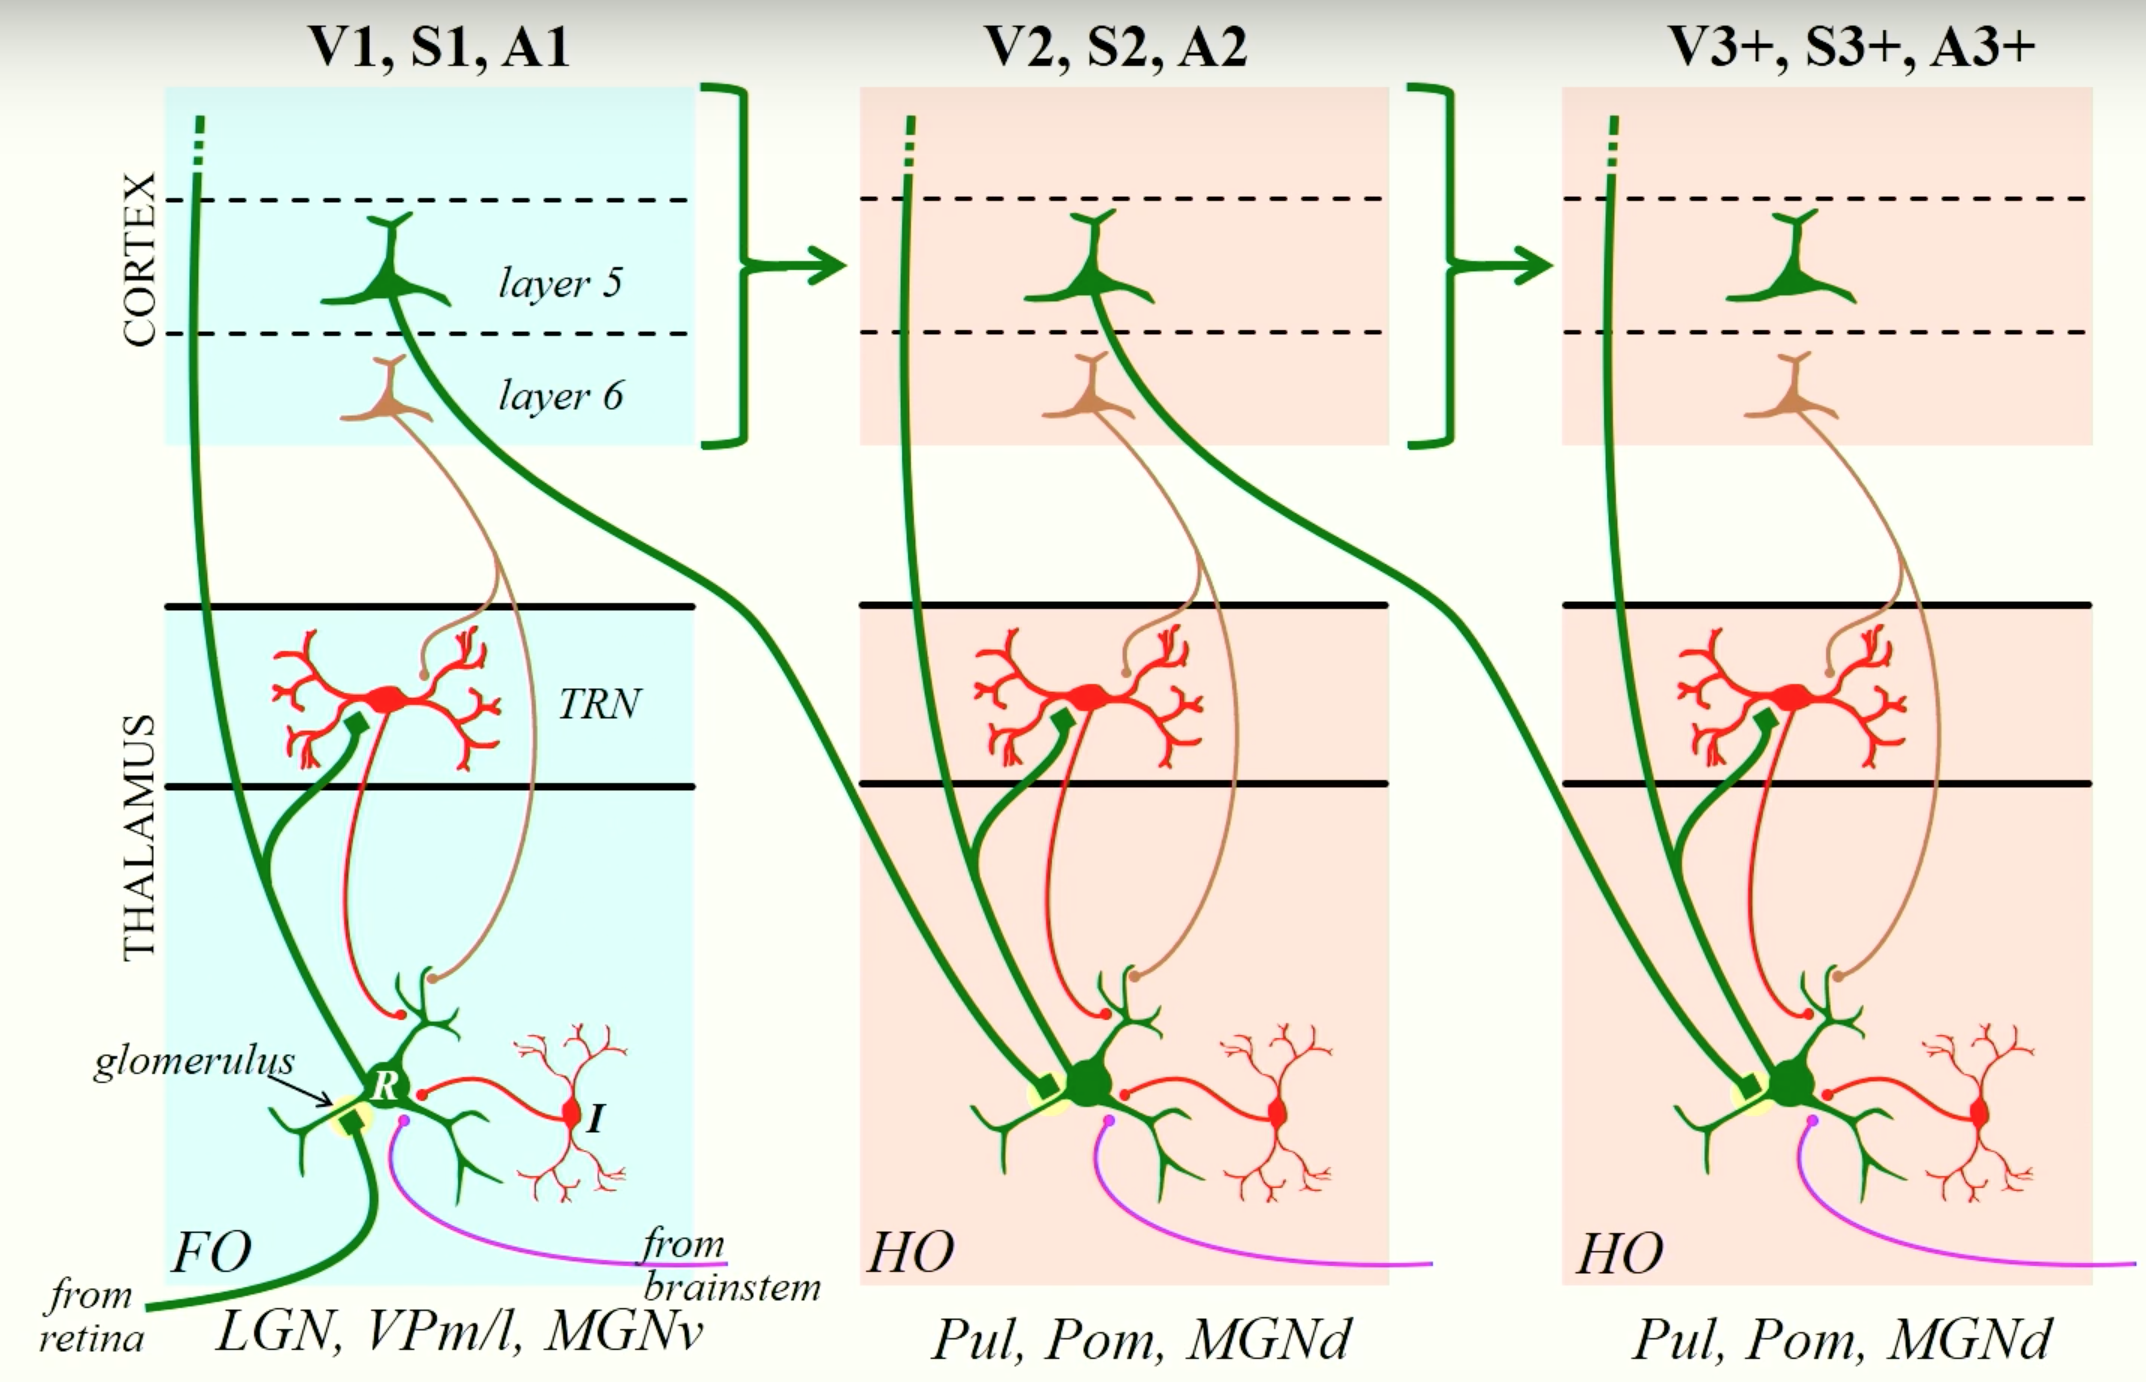
\includegraphics[width=\textwidth]{images/neuroscience/thalamocortical_circuits.png}
        \caption{ }
        \label{fig: thalamocortical circuits}
    \end{subfigure}%
    ~ 
    \begin{subfigure}[t]{0.5\textwidth}
        \centering
        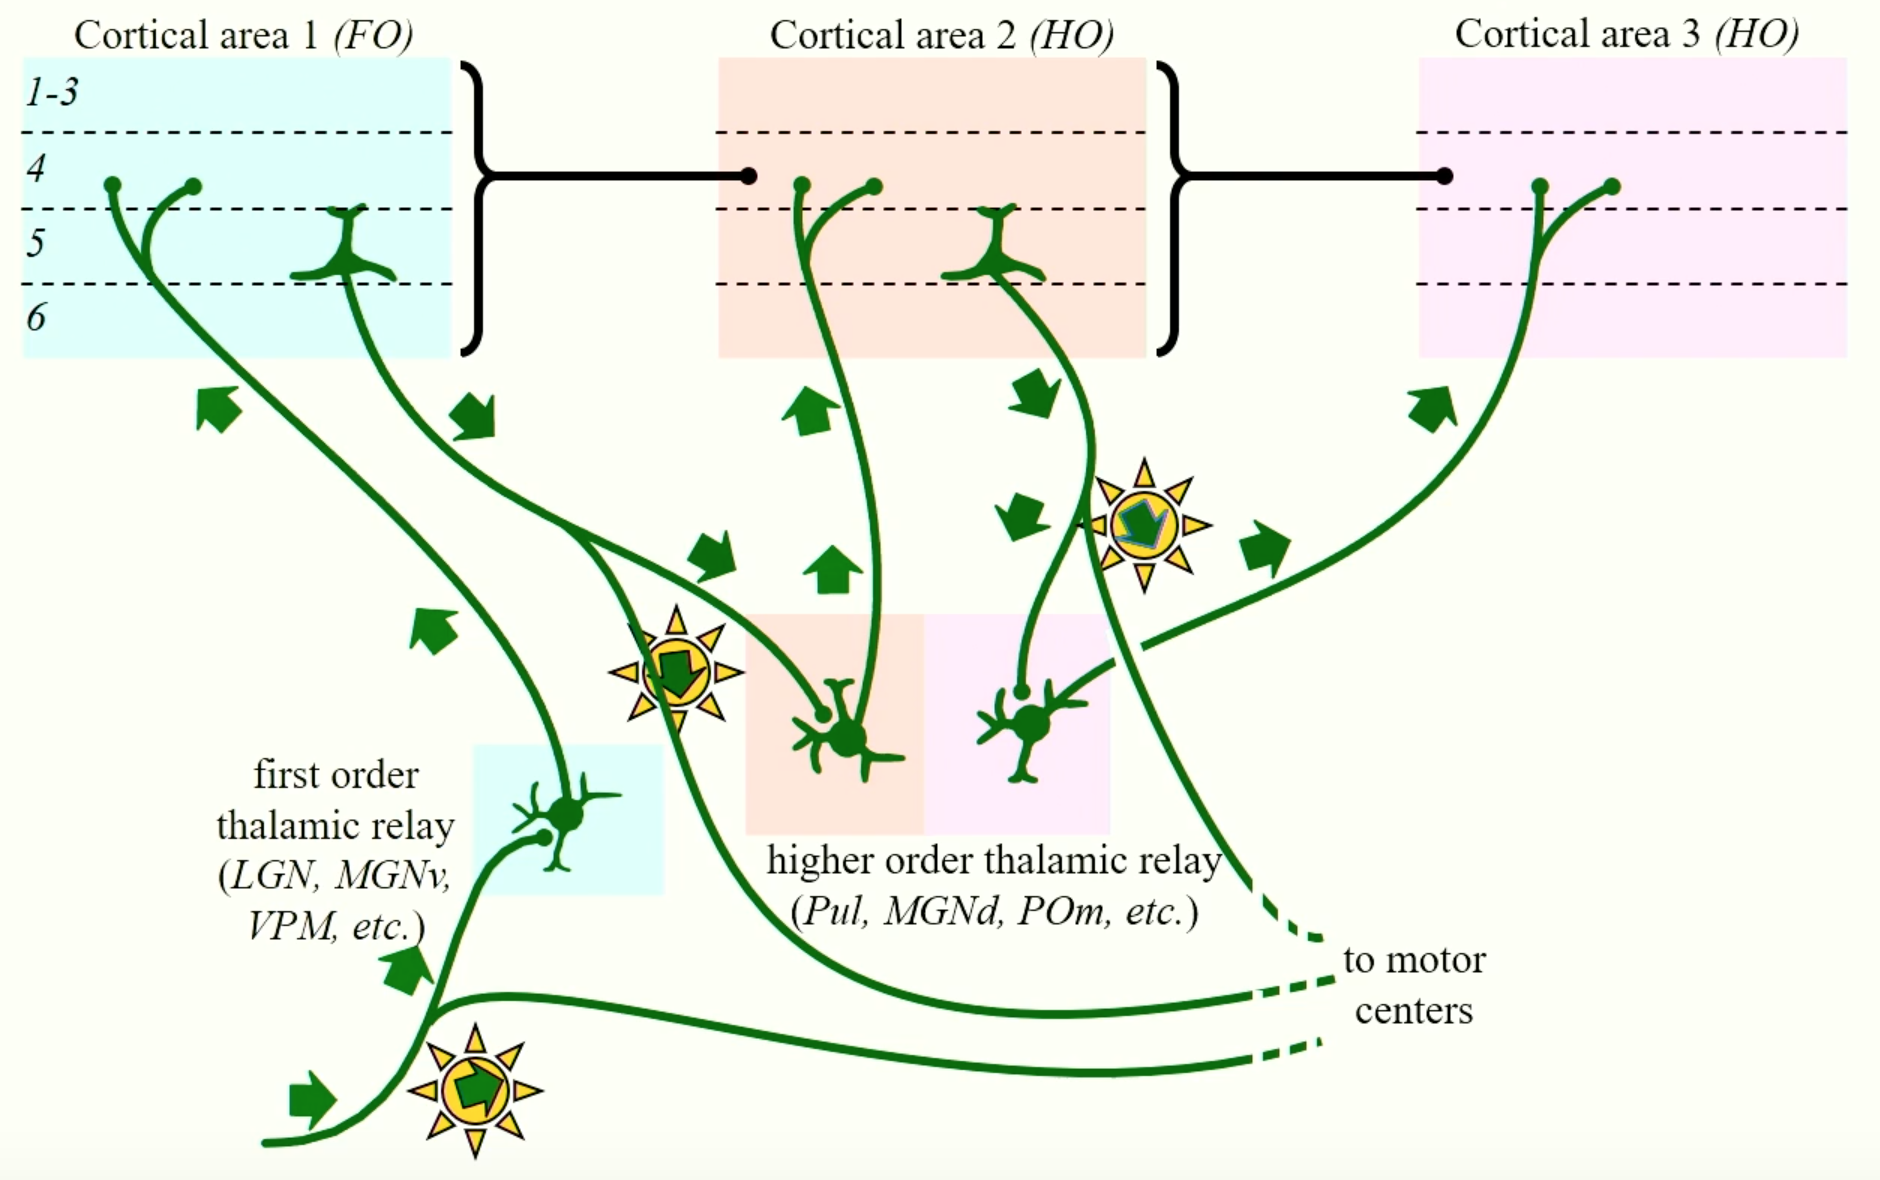
\includegraphics[width=\textwidth]{images/neuroscience/thalamus_branching_axons.png}
        \caption{ }
        \label{fig: thalamus branching axons}
    \end{subfigure}
    \caption{(\textbf{a}) Basic circuit diagram of first-order (left) and higher-order (center, right) thalamocortical circuits across multiple sensory modalities. (\textbf{b}) Cortical cells that project to thalamus often have branching axons that also project to sub-cortical motor centers. Reproduced from S. Murray Sherman.}
\end{figure*}


\section{Neocortical Circuits}

A review of various experimental findings on cortical circuits is presented in \cite{harris2015neocortical}. While there are differences in cortical structure and activity across different areas and species, many cortical circuit properties are conserved. \cite{harris2015neocortical} therefore argues that these differences are \textit{quantitative} rather than \textit{qualitative}, arising from differences in gene expression and inputs. They refer to these slight differences on a main conserved architecture as \textit{serial homology}. The primary categorization of neocortical neurons is between excitatory cells (EC), which constitute roughly $80\%$ of neurons, and interneurons, which constitute the remaining $20\%$.  

A somewhat more simplistic view, with a focus on predictive coding, is presented in \cite{bastos2012canonical}.

\subsubsection{Excitatory Cells}

Excitatory cells are classified into three main categories:
\begin{itemize}
	\item \textbf{intratelencephalic (IT) neurons}: Found in layers 2-6 and project axons only within the telecephalon (neocortex, striatum, and corticoid structures such as amygdala and claustrum). They are the only ECs that project to contralateral cortex. There are many distinct subclasses of IT cells, such as those found in L4.
	\item \textbf{pyramidal tract (PT) neurons}: These are large pyramidal neurons found in layer 5B that project to subcerebral targets including brain stem, spinal cord and midbrain, as well as thalamus and striatum. 
	\item \textbf{corticothalamic (CT) neurons}: Found in layer 6 and project primarily to ipsilateral thalamus.
\end{itemize}
Morphologies of these cell types are shown in Figure \ref{fig: cortical morphologies}. It should be noted that all class of ECs form recurrent connections with local neurons of the same class. Across classes, however, the connectivity is asymmetric, which has led to the hypothesis of a sequential circuit organization. This sequence is typically understood in terms of
$$ \text{thalamus} \rightarrow \text{L4 IT neurons} \rightarrow \text{Other IT neurons} \rightarrow \text{PT neurons},$$
with the role of CT neurons within the circuit still largely unknown. 

\begin{figure}[h]
    \centering
    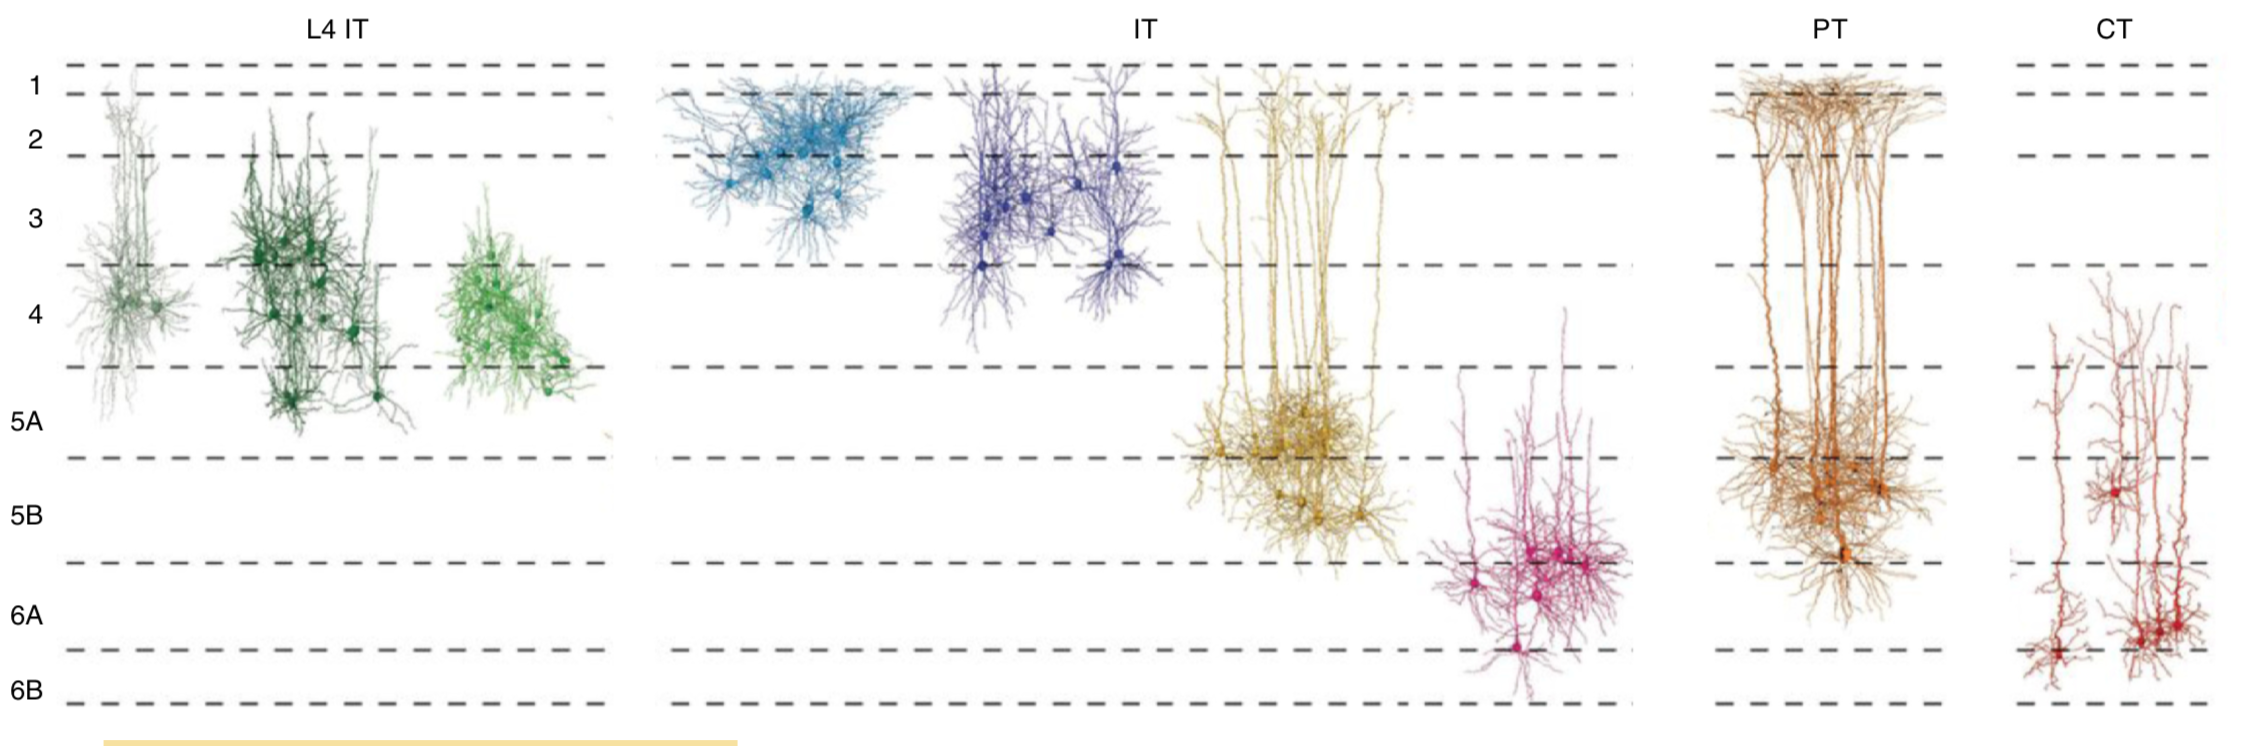
\includegraphics[width=\textwidth]{images/neuroscience/cortical_morphologies.png}
    \caption{Morphologies of various classes of excitatory cells in neocortex. Reproduced from \cite{harris2015neocortical}.}
    \label{fig: cortical morphologies}
\end{figure}

Most of the subcortical inputs to the cortex arise from thalamus and are roughly divided into ``core" and ``matrix" connections. The core relay neurons carry rapid sensory or motor information and are located in primary relay nuclei. These axons tend to form topographic connections in L4 or primary sensory areas. The matrix relay neurons are not well understood, but are typically found in higher order nuclei and project to L1 (and sometimes other layers) of one or more cortical areas. The core-matrix distinction applies most directly to primary sensory areas, but is also found in motor areas and possibly other areas. Higher order sensory cortex, for instance, receives predominantly matrix-type thalamocortical (TC) connections. 

L4 neurons are a special case of IT neurons. They project asymmetrically to L2/3 and L5, and are therefore considered ``upstream" of other circuit components. There are many morphological subclasses of L4 IT neurons, but they largely have similar circuit properties. Layer 4 is enlarged in primary sensory areas, so L4 neurons are thought to be specialized for sensory processing, with different sensory areas tuned appropriately. In higher-order sensory areas, L4 receives input from thalamus as well as lower areas of cortex. Although motor areas appear to lack a well defined L4, they may contain L4 type cells. 

Other IT neurons receive input from L4 neurons and TC connections. Their outputs project to distant neocortical and striatum areas as well as locally to PT and CT neurons. L2 IT neurons receive matrix-type TC input and inputs from L5A and L4. L3 IT neurons receive similar inputs, with the addition of core-type TC inputs. These neurons tend to exhibit sparse firing and project to L5. The L5 IT neurons tend to be reciprocally connected to L2/3 and also have broad range connections, particularly to striatum. L6 IT neurons are less studied but tend to make distant connections. 

PT neurons receive cortical (L2/3) and TC (core-type) input and project to specialized subcortical areas, such as spinal or tectal areas. They also make connections with ipsilateral cortex and thalamus. They tend to display bursting firing patterns, which provide a ``dense code." This is perhaps an information-theoretic adaptation to broadcast cortical output through a small number of channels. 

CT neurons are found in L6, and tend to receive input from higher-order cortical areas, as well as some input from thalamus. Their projections to thalamic areas are slow and weak, so they are often considered as modulators instead of drivers. It is thought that CT neurons may integrate long-range cortical inputs to modulate TC activity, acting as a sort of gain control. 

\begin{figure}[h]
    \centering
    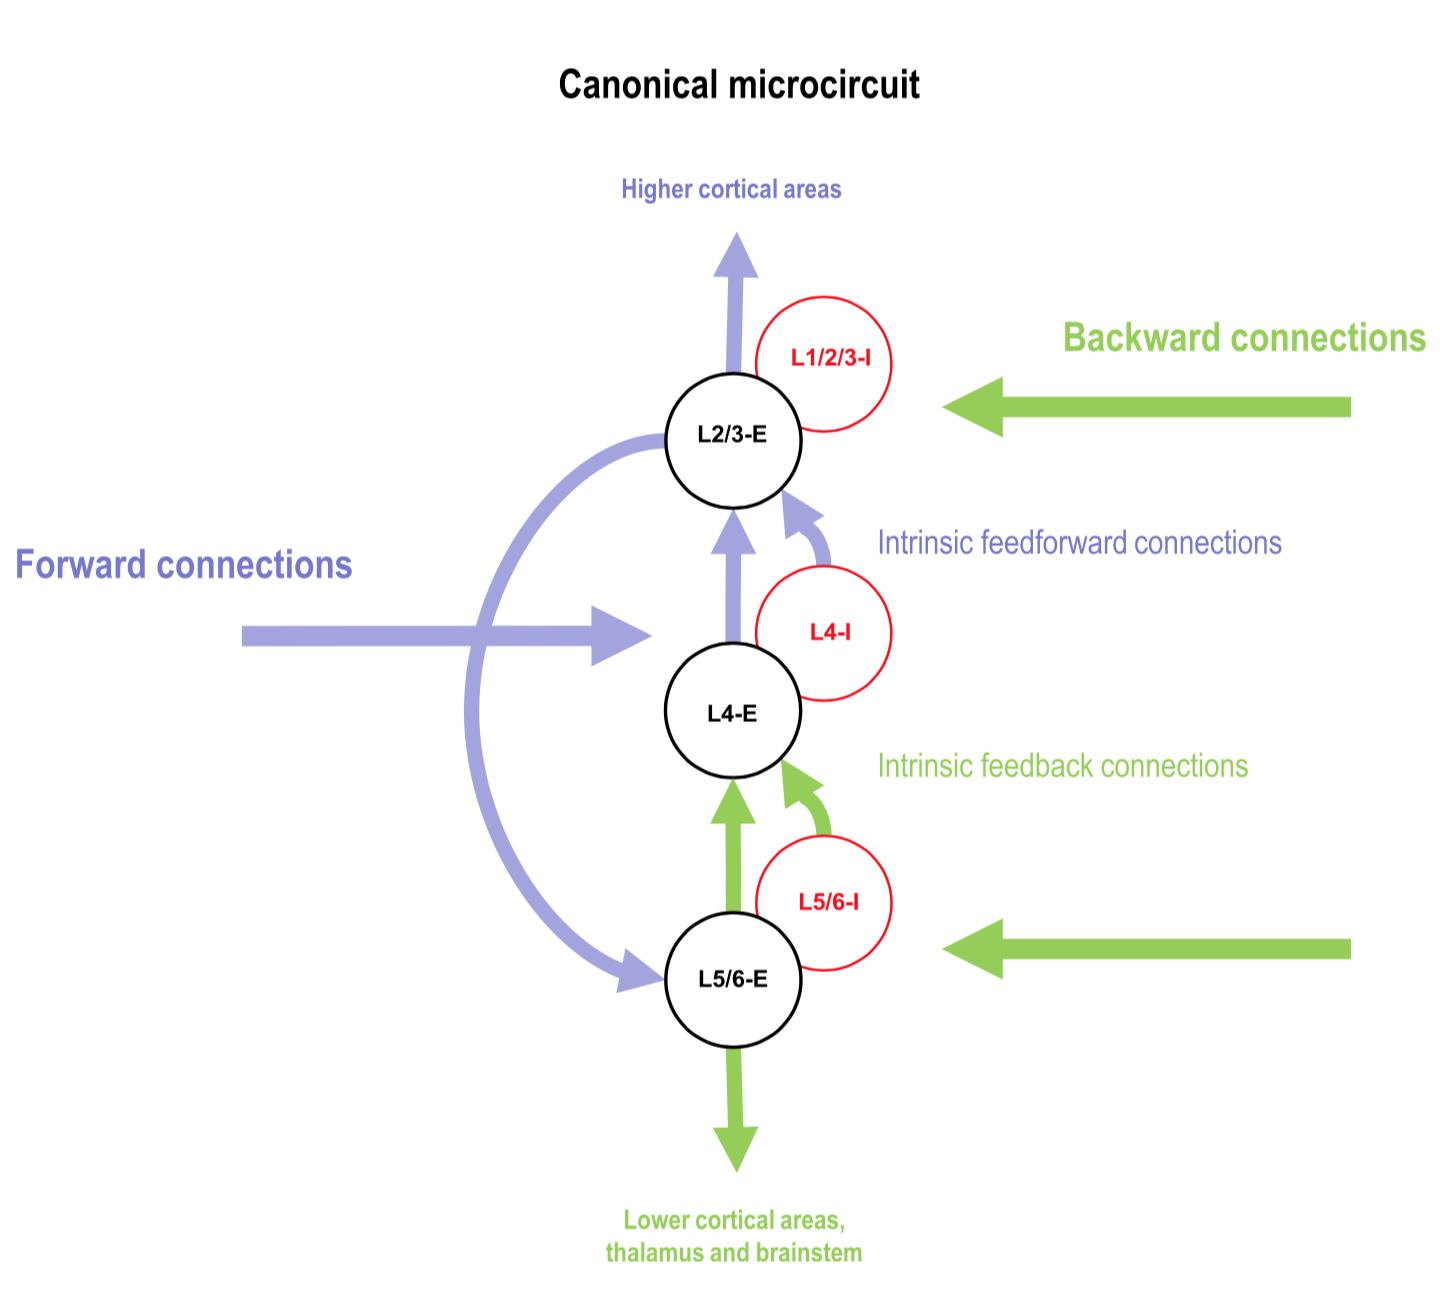
\includegraphics[width=0.75\textwidth]{images/neuroscience/pc_connectivity.png}
    \caption{Connectivity diagram for a cortical microcircuit. Reproduced from \cite{bastos2012canonical}.}
    \label{fig: pc connectivity}
\end{figure}

\subsubsection{Interneurons}

Cortical interneurons are categorized into three classes based on gene expression:
\begin{itemize}
	\item \textbf{Pvalb}
	\item \textbf{Sst}
	\item \textbf{Htr3a}
\end{itemize}
Interneurons contain many subclasses, which inhibit various local ECs and other interneurons. These inhibitory circuits may mediate diverse control of cortical processing during behavior, at least partially contributing to the quantitative differences between cortical circuits that perform different computations, yet have similar qualitative architectures. 


\chapter{Computational Theories of Neuroscience}
\label{chap: computational theories of neuroscience}

\section{Introduction}


\section{Integrate \& Fire Neurons}



\section{Canonical Neural Computations}

\subsection{Linear Weighting}


\subsection{Exponentiation}


\subsection{Normalization}

Normalization is a useful operation, ubiquitous in both biological nervous systems and machine learning systems. \cite{carandini2012normalization} reviews various forms of normalization that appear in different brain areas and species. They define (divisive) normalization as \textit{the computation in which the responses of neurons are divided by a common factor that typically includes the summed activity of a pool of neurons}. They point to examples of normalization in olfactory pathways, retinal contrast adaptation, V1, MT, V4, IT, medial superior temporal area (MST), auditory cortex, and lateral intraparietal area (LIP). They also point to a role of normalization in mediating attentional mechanisms, such as winner-take-all competition. The authors offer a number of reasons for the ubiquity of normalization, i.e. possible uses:
\begin{itemize}
	\item \textbf{Maximizing Sensitivity}: adjusting the gain of neural responses to stay within the dynamic range.
	\item \textbf{Invariance}: discarding mean activation information and various irrelevant features
	\item \textbf{Neural Decoding}: treating a population of neurons as a normalized probability distribution
	\item \textbf{Stimuli Discrimination}: making discrimination easier for a linear classifier
	\item \textbf{Max Pooling}: biased and winner-take-all competition
	\item \textbf{Redundancy Reduction}: increasing the efficiency of neural representations by creating statistically independent activations.
\end{itemize}
Normalization is implemented in various circuits using various biophysical mechanisms, such as inhibition (polarization modulation), shunting inhibition (conductance modulation), and synaptic depression. Across many implementations, the overall computational scheme appears to rely on a ``summation field" and a ``suppression field," in which the activity of the summation field is divisively normalized according to the suppression field.


\section{Action Selection}

A theory put forth by \cite{daw2005uncertainty} discusses two complementary pathways for action selection. The first, shorter pathway involves a state-value look-up, hypothesized to use striatum. This is thought to correspond to model-free, value-based methods in reinforcement learning. The second, longer pathway involves explicit planning through evaluation of possible future outcomes, likely using prefrontal cortex. This is thought to correspond to model-based learning.

\chapter{Predictive Coding}

\section{Introduction}

Predictive coding, in its current form, was formalized by \cite{rao1999predictive}. This theoretical neuroscience model posited that sensory processing is a filtering problem, in which latent states underlying the environmental stimuli are estimated according to their agreement with the observed input as well as prior beliefs about these quantities. This offered an explanation for ``extra-classical" receptive field effects in visual processing, in which stimuli outside the receptive field of a particular cortical neuron are able to affect that neuron's activity. This was explained as the result top-down prior beliefs.

However, the notion of perception as a generative process dates back to at least \cite{von1867handbuch}. \textit{TODO: mention other early work before Rao and Ballard with similar ideas}

Predictive coding claims that sensory processing, i.e. perception, is fundamentally about constructing a generative model of the input sensory signal. To perform \textit{inference} in this model (to perceive), the model uses its current estimate of the latent variables underlying the environment to generate reconstructions or predictions of the input. Using the residual (error) from this reconstruction or prediction, along with residuals from prior beliefs, the model updates its estimate of these latent variables. \textit{Learning} corresponds to updating the parameters of the generative model to improve these overall residuals.
\newline

\subsection{Literature Summary}

\noindent \cite{clark2013whatever} provides a survey of the area of predictive coding
\newline

\noindent \cite{friston2002functional, friston2003learning, friston2005theory} presents a free energy formulation of predictive coding that uses expectation maximization. Primarily focuses on the static setting. Puts forth a theory of cortical processing as carrying out predictive coding.
\newline

\noindent \cite{friston2003dynamic} presents \textit{dynamic causal modeling}.
\newline

\noindent \cite{friston2008variational} presents \textit{variational filtering}.
\newline

\noindent \cite{friston2008DEM} presents \textit{dynamic expectation maximization} (DEM).
\newline

\noindent \cite{friston2010generalised} presents \textit{generalized filtering}, which does not make the mean-field assumption and instead treats all unknown variables as conditionally dependent. This differs from variational filtering \cite{friston2008variational} in that it assumes the parameters and precisions also change with time, with a prior on smoothness of these changes.
\newline

\noindent \cite{feldman2010attention} claims that attention can be formulated as the adjustment of prior precisions in the predictive coding model.
\newline

\noindent \cite{friston2011action}, \cite{friston2013anatomy} , \cite{friston2015active} \cite{friston2016active_process}, \cite{friston2016active} discuss \textit{active inference}.
\newline

\section{The Static Setting}

\subsection{MAP State Estimation in a One--Level Model}

Consider a situation in which the value of a single latent variable $z$ must be inferred from a single observed variable $x$. This is represented by the graphical model in figure  \ref{fig: simple_latent_model}. Let $g$ denote a non-linear function defining how $z$ generates $x$. Assume that the generated output takes the form of a normal distribution with mean $\mu_x = g(z)$ and constant variance $\sigma^2_x$:

\begin{figure}
    \centering
    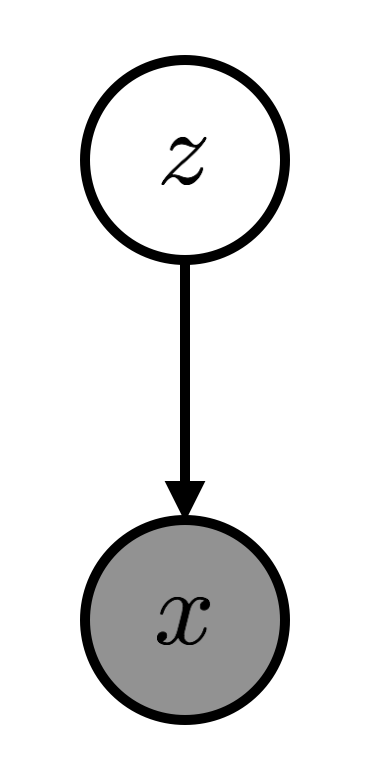
\includegraphics[width=0.15\textwidth]{images/predictive_coding/simple_latent_graphical_model.png}
    \caption{A graphical model denoting a latent variable model in which a single latent variable $z$ generates a single observed variable $x$. In predictive coding, we typically assume that $p(z)$ and $p(x|z)$ are Gaussian densities, and the generative mapping from $z$ to $x$ is a non-linear function.}
    \label{fig: simple_latent_model}
\end{figure}

\begin{equation}
	p (x | z) = \mathcal{N} (x; g(z), \sigma^2_x).
\end{equation}

\noindent Recall that in one dimension, a normal distribution takes the form

\begin{equation}
	\mathcal{N} (x; \mu, \sigma^2) = \frac{1}{\sqrt{2 \pi \sigma^2}} e^{-\frac{(x - \mu)^2}{2 \sigma^2}}.
	\label{eq: 1d gaussian}
\end{equation}

\noindent We will place a prior on $z$, which we also assume is a normal distribution with constant mean $\mu_p$ and constant variance $\sigma^2_p$:

\begin{equation}
	p (z) = \mathcal{N} (z; \mu_p, \sigma^2_p).
\end{equation}

\noindent To infer the posterior distribution of $z$, we can use Bayes' rule to invert the generative model:

\begin{equation}
	p (z | x) = \frac{p(x | z) p(z)}{p(x)},
\end{equation}

\noindent where the marginal distribution in the denominator is given as

\begin{equation}
	p (x) = \int p(x | z) p(z) dz.
	\label{eq: intractable integration}
\end{equation}

In general, computing the exact posterior distribution is computationally intractable due to the integration over $z$ in eq. \ref{eq: intractable integration}. Instead, we'll resort to variational inference\footnote{We are not actually using variational inference here, since the maximum of $p(z | x)$ must also be the maximum of $p(x, z)$ through the definition of conditional probability: $p(z|x) = \frac{p(x, z)}{p(x)}$, since $p(x)$ does not depend on the value of $z$. } to find the maximum (mode) of the posterior, otherwise known as the maximum a posteriori or MAP estimate. This is the \textit{most likely} estimate of the value of $z$. We will define our approximate distribution, a point mass estimate at $\mu_q$, as $q(z|x) = \delta (z = \mu_q)$, with the MAP estimate denoted as $\hat{\mu}_q$.

We want to maximize the evidence lower bound (ELBO), $\mathcal{L}$:

\begin{equation}
	\mathcal{L} = \mathbb{E}_{z \sim q(z|x)} \left[ \log p(x, z) - \log q(z|x) \right] = \mathbb{E}_{z \sim q(z|x)} \left[ \log p(x|z) + \log p(z) - \log q(z|x) \right] 
	\label{eq: elbo 1}
\end{equation}

\begin{equation}
	\mathcal{L} = \log \left( \frac{1}{\sqrt{2 \pi \sigma_x^2}} e^{-\frac{(x - g(\mu_q))^2}{2 \sigma_x^2}} \right) + \log \left( \frac{1}{\sqrt{2 \pi \sigma_p^2}} e^{-\frac{(\mu_q - \mu_p)^2}{2 \sigma_p^2}} \right)
	\label{eq: elbo 2}
\end{equation}

\begin{equation}
	\mathcal{L} = -\frac{1}{2} \log ( 2 \pi \sigma_x^2 )  - \frac{(x - g(\mu_q))^2}{2 \sigma_x^2} - \frac{1}{2} \log ( 2 \pi \sigma_p^2 ) -\frac{(\mu_q - \mu_p)^2}{2 \sigma_p^2}
	\label{eq: elbo 3}
\end{equation}

\begin{equation}
	\mathcal{L} = \frac{1}{2} \left( - \log ( \sigma_x^2 )  - \frac{(x - g(\mu_q))^2}{\sigma_x^2} - \log ( \sigma_p^2 ) -\frac{(\mu_q - \mu_p)^2}{\sigma_p^2} \right) + \text{const.}
	\label{eq: elbo 4}
\end{equation}

\noindent In going from eq. \ref{eq: elbo 1} to eq. \ref{eq: elbo 2}, we used the fact that $q(z|x)$ is a delta function, so the expectation becomes an evaluation at a single point, $z=\mu_q$. The expectation of $q(z|x)$ at this point is $1$, so $\log q(z|x)$ evaluates to $0$. To find the MAP estimate, we must solve the following optimization problem:

\begin{equation}
	\hat{\mu}_q = \text{argmax}_{\mu_q} \mathcal{L} =  \text{argmax}_{\mu_q} \frac{1}{2} \left( - \log ( \sigma_x^2 )  - \frac{(x - g(\mu_q))^2}{\sigma_x^2} - \log ( \sigma_p^2 ) -\frac{(\mu_q - \mu_p)^2}{\sigma_p^2} \right).
\end{equation}

\noindent To use first-order optimization methods, we must find the partial derivative of $\mathcal{L}$ w.r.t. $\mu_q$:

\begin{equation}
	\frac{\partial \mathcal{L}}{\partial \mu_q} = \frac{x - g(\mu_q)}{\sigma_x^2} \frac{d g}{d \mu_q} + \frac{\mu_q - \mu_p}{\sigma_p^2}
	\label{eq: 1d gradient}
\end{equation}

\noindent We see that we have two terms: \textbf{the first term moves the estimate toward agreement with the observation}, and \textbf{the second term moves the estimate toward agreement with the prior}. Each of these terms are weighted by their corresponding variances. In other words, inference (i.e. finding the optimal estimate of $\mu_q$) involves a weighted combination of \textit{bottom-up} and \textit{top-down} information. By repeatedly moving our estimate $\mu_q$ along this gradient, we can hopefully arrive at the MAP estimate $\hat{\mu}_q$. Note that we may not find the true value $\hat{\mu}_q$ if the optimization surface is non-convex. 

We would like to extend this single dimensional model to handle latent and observed variables of arbitrary size. In this setting, $\mathbf{x}$ and $\mathbf{z}$ are now vectors. The conditional likelihood, $p(\mathbf{x} | \mathbf{z}) = \mathcal{N} (\mathbf{x}; \bm{\mu}_\mathbf{x} = g(\mathbf{z}), \bm{\Sigma}_\mathbf{x})$ is now a multi-variate Gaussian distribution. The general form for this distribution is

 \begin{equation}
	\mathcal{N} (\mathbf{x}; \bm{\mu}, \bm{\Sigma}) = \frac{1}{(2 \pi)^{n/2} | \bm{\Sigma}|^{1/2}}  e^{-\frac{1}{2}(\mathbf{x} - \bm{\mu})^\intercal \bm{\Sigma}^{-1}(\mathbf{x} - \bm{\mu})},
	\label{eq: multi-variate gaussian}
\end{equation}

\noindent where $\bm{\Sigma}$ is the covariance matrix, $| \bm{\Sigma}|$ is the determinant of $\bm{\Sigma}$, and $n$ is the dimensionality of the vector $\mathbf{x}$. The prior on $\mathbf{z}$ is also a multi-variate Gaussian: $p(\mathbf{z}) = \mathcal{N} (\mathbf{z}; \bm{\mu}_p, \bm{\Sigma}_p)$. The MAP estimate is now a vector, $\hat{\bm{\mu}}_q$, of the most likely estimate of $\bm{\mu}_q$. To find this estimate, we must again optimize $\mathcal{L}$ w.r.t. $\bm{\mu}_q$. Repeating the steps above, the gradient, $\nabla_{\bm{\mu}_q} \mathcal{L}$, is given as:

\begin{equation}
	\nabla_{\bm{\mu}_q} \mathcal{L} =  \left( \frac{d g}{d \bm{\mu}_q} \right)^\intercal \bm{\Sigma}^{-1}_\mathbf{x} (\mathbf{x} - g(\bm{\mu}_q)) + \bm{\Sigma}^{-1}_p (\bm{\mu}_q - \bm{\mu}_p).
	\label{eq: multi-dimensional gradient}
\end{equation}

\section{The Dynamic Setting}

\section{Attention}

\section{Active Inference}

\section{Neural Implementation}

\subsection{Correspondence with Cortical Mircrocircuits}

\noindent \cite{bastos2012canonical} outlines ideas about correspondence between predictive coding and cortical microcircuits.
\newline

\noindent \cite{kanai2015cerebral} proposes that the pulvinar region of the thalamus is involved in setting precisions of predictions.
\newline

\noindent \cite{bogacz2017tutorial} gives an introductory tutorial to predictive coding with ideas about implementing predictive coding in neocortex.
\newline

\noindent \cite{whittington2017approximation} draws comparisons between backprop and predictive coding.
\newline



\part{Machine Learning}
\chapter{Neural Networks}
\section{Basics}


\subsection{Linear Threshold Units}

\subsection{Multi-Layer Perceptrons}

\subsection{Backpropagation}


\chapter{Representation Learning}

\section{Introduction}

\textit{Representation learning} is the process of taking data, $\mathbf{x}$, and forming a representation, $\mathbf{z}$, that captures the ``meaningful" information contained in the data. How do we define what constitutes meaningful information? This question exposes a fundamental aspect of representation learning: it is inherently ill-defined. There is no way in which to truly assess the quality of a representation, i.e. which aspects of the data are meaningful, without defining a \textit{task}, $\mathbf{y}$, which one hopes to accomplish with the representation. In Section \ref{sec: information bottleneck}, we discuss the information bottleneck theory \cite{tishby2000information}, an information theoretic framework for representation learning. Then, in Section \ref{sec: representation learning without a task}, we discuss learning representations in the absence of a clearly defined task, where we outline a variety of heuristics and priors.

\section{The Information Bottleneck}
\label{sec: information bottleneck}

The \textbf{information bottleneck} is a compression method that squeezes the information that an input variable $\mathbf{x} \in X$ (data) contains about some other variable $\mathbf{y} \in Y$ (task) through a `bottleneck' formed by a representation $\mathbf{z} \in Z$ \cite{tishby2000information}. The approach is motivated by rate distortion theory \cite{cover2012elements}, in which the quality of a representation is determined by
\begin{enumerate}
	\item the \textit{information rate}, i.e. the average amount of information required to specify $\mathbf{z}$ without confusion
	\item the \textit{distortion function} $d$, which implicitly specifies the most relevant aspects of the input $X$. 
\end{enumerate}
\noindent A good representation is thus one that maximally compresses the meaningful information in the data. We could solve for the representation by introducing a Lagrange multiplier $\beta$ and use variational methods to solve the following equation for $p(\mathbf{z}|\mathbf{x})$:
\begin{equation}
	\mathcal{F} [p(\mathbf{z}|\mathbf{x})] = I(Z; X) + \beta \langle d(\mathbf{z}, \mathbf{x}) \rangle_{p(\mathbf{z}|\mathbf{x})},
\end{equation}
\noindent where $I$ denotes the mutual information. However, we rarely have access to the correct distortion function. The information bottleneck method instead uses another variable $Y$ to specify the relevant aspects of $X$. The tradeoff between compression and information preservation is expressed by the functional
\begin{equation}
	\mathcal{L} [p(\mathbf{z}|\mathbf{x})] = I(Z; X) - \beta I(Z; Y).
\end{equation}
\noindent An exact formal solution can be derived for this functional. One can solve the free-energy functional
\begin{equation}
	\mathcal{F}[p(\mathbf{z} | \mathbf{x}), p(\mathbf{z}), p(\mathbf{y} | \mathbf{z})] = I(Z; X) + \beta \langle D_{KL} (p(\mathbf{y} | \mathbf{x}) || p(\mathbf{y} | \mathbf{z}) ) \rangle_{p(\mathbf{x}, \mathbf{z})}
\end{equation}
\noindent for $p(\mathbf{z} | \mathbf{x})$, $p(\mathbf{z})$, and $p(\mathbf{y} | \mathbf{z})$, using a deterministic annealing approach for $\beta$. Building on this work, in \cite{achille2017emergence}, an ideal representation is defined as one that is:
\begin{enumerate}
	\item \textbf{sufficient}: capturing the information contained in $\mathbf{x}$ that is sufficient to estimate $\mathbf{y}$, i.e. $I(Y; Z) = I(Y; X)$.
	\item \textbf{minimal}: retains as little information about $\mathbf{x}$ as possible, making the task easier, i.e. $I(Z; X)$ is minimized.
	\item \textbf{invariant}: nuisances $n$ have no effect on the representation, which helps to prevent overfitting i.e. $I(Z; n) = 0$.
	\item \textbf{disentangled}: the total correlation, defined as the dissimilarity between the representation and the product of its marginals, $TC(\mathbf{z}) \equiv D_{KL} (p(\mathbf{z}) || p(\mathbf{z}_1) p(\mathbf{z}_2) \dots p(\mathbf{z}_L))$, is minimized.
\end{enumerate}

\noindent It is shown that only (1) and (2) need to be enforced, as (3) and (4) naturally follow.


\section{Representation Learning Without a Task}
\label{sec: representation learning without a task}

Often, we do not have a well-defined task, however, we would still like to learn a representation that captures aspects of the data that will facilitate rapid transfer learning to future tasks. This is referred to as \textit{unsupervised learning}. The lack of task implies that we no longer have a measure of sufficiency, meaning that we must define an alternative quantity to optimize. 

\cite{bengio2013representation} identify an alternative set of \textit{priors} for ideal representations:

\begin{enumerate}
	\item \textbf{smoothness}: the representation should be a \textit{smooth} mapping of the data, i.e. if $\mathbf{x}^{(1)} \approx \mathbf{x}^{(2)}$, then $\mathbf{z}^{(1)} \approx \mathbf{z}^{(2)}$.
	\item \textbf{multiple explanatory factors}: the representation is made up of a set of disentangled factors that explain the data. This is also sometimes referred to as a distributed representation.
	\item \textbf{hierarchical organization}: the representation is arranged in a hierarchy from lower level to more abstract factors.
	\item \textbf{semi-supervised}: the factors necessary for modeling the data $\mathbf{x}$ are useful for modeling some task labels $\mathbf{y}$. This is related to sufficiency mentioned above, but does not place importance on the task first and foremost.
	\item \textbf{shared factors across tasks}: explanatory factors within the representation should be useful more multiple tasks
	\item \textbf{manifolds}: probability mass should be concentrated near regions that are much smaller than the entire dimensionality of the data. The data does not occupy the input space uniformly.
	\item \textbf{natural clustering}: different explanatory factors may lie on different manifolds.
	\item \textbf{temporal and spatial coherence}: inputs that are nearby in space and time should be similar (although this can be violated)
	\item \textbf{sparsity}: only a small number of factors within the representation should be active for any particular data example.
	\item \textbf{simplicity of factor dependencies}: the higher level factors should have simple (i.e. linear) dependencies.
\end{enumerate}

\section{Disentangled Representations}

Define disentanglement. Why are disentangled representations helpful? Trade off between disentanglement and faithfully representing the data. How do we learn disentangled representations, while at the same time, respecting the structure of the latent space? Importance of priors.

Two random variables are \textbf{independent} if their joint probability can be expressed as the product of their marginals:

\begin{equation}
	p(\mathbf{x}, \mathbf{y}) = p(\mathbf{x}) p(\mathbf{y}),
\end{equation}

\noindent and they are \textbf{conditionally independent} if their conditional joint probability can be expressed as

\begin{equation}
	p(\mathbf{x}, \mathbf{y} | \mathbf{z}) = p(\mathbf{x} | \mathbf{z}) p(\mathbf{y} | \mathbf{z}).
\end{equation}

Independence is related to covariance, but is a stronger property. Two variables that are independent have zero covariance and two variables that have non-zero covariance are dependent. Zero covariance implies that the variables have no \textit{linear} dependence. Independence implies that the variables also have no \textit{non-linear} dependence. That is, it is possible for two dependent variables to have zero covariance. 


\section{Other}
\noindent \textbf{Notes:}

\cite{cheung2014discovering} propose using a cross-covariance penalty term in the setting of semi-supervised learning of the form:

\begin{equation}
	C(\hat{\mathbf{y}}^{1 \dots N}, \mathbf{z}^{1 \dots N}) = \frac{1}{2} \sum_{ij} \left[ \frac{1}{N} \sum_n (\hat{y}^n_i - \bar{\hat{y}}_i) (z^n_j - \bar{z}_j) \right]^2,
\end{equation}

\noindent where $\hat{\mathbf{y}}$ is a vector of (one-hot) inferred labels and $\mathbf{z}$ is a latent representation. $N$ is the batch size.


\cite{higgins2016early} propose to use a regularization weight in a VAE setting to ``upweight" the amount of regularization as a means of promoting \textbf{redundancy reduction and independence} among the latent representation. They also argue for the importance of \textbf{dense sampling of the (continuous) data manifold} for disentanglement. Sparse sampling of the data manifold results in ambiguity is the manifold interpretation, requiring additional supervision for disentanglement.

\cite{siddharth2016inducing} use supervision to impose structure on part of the latent representation in a VAE.

Dropout \cite{srivastava2014dropout} is a technique for preventing ``fragile coadaptation" between units within a representation, effectively enforcing that they represent different (independent) quantities. This technique also results in redundancy within the representation.
\chapter{Reinforcement Learning}
\label{chap: reinforcement learning}

\section{The RL Problem Setting}

TODO: image of agent environment interaction.

\subsection{The Basics}

Reinforcement learning involves an \textbf{agent} interacting within an \textbf{environment}. The agent selects actions, and the environment responds with new states and rewards. Sutton \& Barto \cite{sutton1998reinforcement} identify four additional sub-elements to reinforcement learning systems:
\begin{itemize}
	\item a \textbf{policy},
	\item a \textbf{reward signal},
	\item a \textbf{value function},
	\item and, optionally, a \textbf{model} of the environment.
\end{itemize}
\noindent A \textit{policy} defines a mapping from (perceived) states to output actions to be taken. A \textit{reward signal} is a real-valued number that the agent receives from the environment. The agent tries to maximize its total reward, which is referred to as value. The \textit{value function} specifies the expected value, starting from a particular state. Thus, it is ultimately value that we try to optimize. Finally, a \textit{model} of the environment is the agent's simulation of the environment, allowing the agent to plan actions and predict outcomes (states, rewards, etc.).

The boundary between agent and environment is often not clearly defined. Sutton \& Barto place the agent-environment boundary at the limit of the agent's control, not at the physical boundary. For instance, the limbs of the agent, its internal energy reserves, and even the reward mechanism are considered to be part of the environment, since the agent does not have absolute control over these aspects.

We assume that time unfolds in a series of discrete time-steps, $t = 1, 2, 3, \dots$ At each time step, the agent is in some state $S_t \in \mathcal{S}$ and chooses some action $A_t \in \mathcal{A} (S_t)$. Here, $\mathcal{S}$ denotes the space of possible states and $\mathcal{A} (S_t)$ denotes the space of possible actions from state $S_t$. The action is chosen based on the agent's policy $\pi_t (a | s)$, which probabilistically maps states $S_t = s$ to actions $A_t = a$. At the next time step, the agent receives a real-valued reward, $R_{t+1} \in \mathcal{R} \subset \mathbb{R}$, and arrives in the next state, $S_{t+1}$.

The \textbf{return}, $G_t$, is the (discounted) sum of rewards starting at time $t$. For \textbf{episodic tasks}, in which the sequence has a finite length, $T$, this is defined as 

\begin{equation}
G_t \triangleq R_{t+1} + R_{t+2} + \dots + R_T = \sum_{k=0}^{T - t - 1} R_{t + k + 1},
\end{equation}

\noindent However, for \textbf{continuing tasks}, in which the time sequence length can be infinite, we include a \textbf{discount rate}, $\gamma \in [0, 1]$, to prevent the return from going to infinity:

\begin{equation}
G_t \triangleq R_{t+1} + \gamma R_{t+2} + \gamma^2 R_{t+3} + \dots = \sum_{k=0}^{\infty} \gamma^k R_{t + k + 1}.
\end{equation}

The \textbf{value function} or \textbf{state-value function}, $v_\pi (s)$, is defined as the expected return from being in state $s$ when using policy $\pi$:

\begin{equation}
	v_\pi (s) \triangleq \mathbb{E}_\pi \left[ G_t | S_t = s \right] = \mathbb{E}_\pi \left[ \sum_{k=0}^{\infty} \gamma^k R_{t + k + 1} | S_t = s \right].
	\label{eq: value_func_def}
\end{equation}

\noindent Note that here we are assuming that the task respects the Markov property; the current state, along with the policy, contains all of the information to determine the value function. We can also define an \textbf{action-value function}, $q_\pi (s, a)$, which specifies expected returns for each action $a$ taken from state $s$ using policy $\pi$:

\begin{equation}
	q_\pi (s, a) \triangleq \mathbb{E}_\pi \left[ G_t | S_t = s, A_t = a \right] = \mathbb{E}_\pi \left[ \sum_{k=0}^{\infty} \gamma^k R_{t + k + 1} | S_t = s, A_t = a \right].
\end{equation}

Using the definition of the value function, we can derive a recursive relationship known as the \textbf{Bellman equation}. Starting from eq. \ref{eq: value_func_def}:

\begin{align}
	\label{eq: bellman_0}
	v_\pi (s) &\triangleq \mathbb{E}_\pi \left[ G_t | S_t = s \right] \\
	\label{eq: bellman_1}
	&= \mathbb{E}_\pi \left[ \sum_{k=0}^{\infty} \gamma^k R_{t + k + 1} \bigg\vert S_t = s \right] \\
	\label{eq: bellman_2}
	&= \mathbb{E}_\pi \left[ R_{t+1} + \gamma \sum_{k=0}^{\infty} \gamma^k R_{t + k + 2} \bigg\vert S_t = s \right] \\
	\label{eq: bellman_3}
	&= \sum_{a, s^\prime, r} \pi(a | s) p(s^\prime, r | s, a) \left[ r + \gamma \mathbb{E}_\pi \left[ \sum_{k=0}^{\infty} \gamma^k R_{t + k + 2} \bigg\vert S_{t+1} = s^\prime \right] \right] \\
	\label{eq: bellman_4}
	&= \sum_{a, s^\prime, r} \pi(a | s) p(s^\prime, r | s, a) \left[ r + \gamma v_\pi (s^\prime) \right].
\end{align}

\noindent To go from eq. \ref{eq: bellman_1} to eq. \ref{eq: bellman_2}, we split the first term out of the sum. To arrive at \ref{eq: bellman_3}, we move the expectation to the future summation, re-expressing the expectation over the first step using summations to weight each return by the appropriate probability of the action $a$, state $s^\prime$, and reward $r$. Finally, to arrive at  \ref{eq: bellman_4}, we notice that the expectation is the value of state $s^\prime$ under our policy, i.e. $v_\pi (s^\prime)$. Thus, we see that the value function has the recursive definition:

\begin{equation}
	v_\pi (s) = \sum_{a, s^\prime, r} \pi(a | s) p(s^\prime, r | s, a) \left[ r + \gamma v_\pi (s^\prime) \right].
\end{equation}

\noindent A similar recursive definition can be derived for $q_\pi (s, a)$.

The \textbf{optimal value function} $v_* (s)$

\subsection{Summary of Notation}


\section{Value Based Methods}

\subsection{Multi-Armed Bandits}

The multi-armed bandit problem is an example of a \textit{non-associative setting}, in which the agent only learns to act in one situation. This simplifies much of the reinforcement learning problem. In particular, the \textbf{multi-armed bandit} problem involves a situation with $k$ possible actions (sometimes referred to as arms, in analogy to slot machines), each with an associated value. The value of action $a$ is denoted as $q_* (a)$, the \textbf{action-value function}. The interaction between the agent and the environment consists of a series of episodes, each of duration 1 time step. At time step $t$, the agent takes \textbf{action} $A_t$ and receives \textbf{reward} $R_t$. Thus, for some action $A_t = a$, the action-value function is defined as

\begin{equation}
	q_* (a) \triangleq \mathbb{E} \left[ R_t | A_t = a \right].
\end{equation}

\noindent Note that rewards can be a stochastic function of the action chosen. $q_* (a)$ encodes the \textit{mean} reward of choosing action $a$. In multi-armed bandit problems, the action-value function is initially unknown. To optimize total reward, we must estimate the action-value function to find the action or actions with the highest reward. Selecting this action will then optimize reward. We refer to the \textbf{action-value estimates} at time step $t$ as $Q_t (a)$.

At any time step $t$, we can either \textbf{exploit} our current knowledge by choosing the action with the optimal action-value estimate, or we can \textbf{explore} other actions with non-optimal action-value estimates. Exploitation is a greedy process, which will likely yield higher rewards in the short-term. Exploration, on the other hand, may find better actions, which can later be exploited, allowing it to likely yield higher rewards in the long-term.

We can select actions according to different strategies. For instance, we could select the action with the optimal action-value estimate at each time step:

\begin{equation}
A_t = \text{argmax}_a Q_t (a)
\end{equation}

\noindent However, this policy will never explore other actions, and may therefore perform poorly in the long run. Another strategy is to select the action with the optimal action-value estimate with probability $1 - \epsilon$ and select a random action with probability $\epsilon$. This strategy is referred to as $\epsilon$\textbf{-greedy}.

\subsection{Dynamic Programming Methods}

\subsubsection{Policy Iteration}

\subsubsection{Value Iteration}

\subsection{Monte Carlo Methods}

\subsection{TD Learning}

\subsubsection{Q Learning}

\subsubsection{SARSA}



\section{Policy Search Methods}
\label{sec: policy search methods}

\subsection{REINFORCE}

\subsection{Actor-Critic Methods}


\section{Deep Reinforcement Learning}
\chapter{Intrinsic Motivation}

\section{Introduction}

Intrinsic motivation is to reinforcement learning as unsupervised learning is to supervised learning. Rather than solely acting to obtain \textit{extrinsic} rewards from the environment\footnote{The concept of rewards being extrinsic is controversial. Indeed, rewards in biological systems are mediated within the system itself. Extrinsic, here, should instead be interpreted as a reward that is directly relevant to performing a task. Intrinsic rewards, on the other hand, are not directly task related.}, the agent also acts to obtain internal \textit{intrinsic} rewards, stemming from learning the environment and the agent's ability to affect the environment. By learning from general purpose signals that connect the perception-action loop, intrinsic motivation can allow an agent to learn how to perceive and act even in environments with sparse or non-existent extrinsic rewards. This \textit{exploration} of the state-action space can facilitate reaching, and ultimately \textit{exploiting}, further extrinsic rewards. In \cite{oudeyer2008can}, the authors characterize intrinsic motivation using the concept of \textit{collative variables} \cite{berlyne1965structure}, which refer to various measures of subjective uncertainty, such as novelty, surprise, ambiguity, complexity, etc., many of which can be expressed in terms of information theoretic quantities. The computational landscape is described in \cite{oudeyer2008can, mirolli2013intrinsically, baldassarre2014intrinsic} as follows:
\begin{enumerate}
	\item \textbf{Knowledge based models} are ``based on measures related to the acquisition of information." \cite{baldassarre2014intrinsic}
	\item \textbf{Competence based models} are based on ``measures related to the learning of skills." \cite{baldassarre2014intrinsic}
	\item \textbf{Morphological models} involve finding relationships between multiple sensorimotor channels which are not based on the agent's long-term knowledge or competence.
\end{enumerate}
A majority of intrinsic motivation approaches fall into the first category, which is the main focus of this chapter. This category has been further subdivided into \textit{prediction}-based approaches and \textit{novelty}-based approaches \cite{mirolli2013intrinsically}. Prediction-based approaches involve forming explicit predictions of future states and inputs, and include measures such as prediction errors \cite{nelson2005finding, barto2004intrinsically}, empowerment \cite{klyubin2005empowerment, mohamed2015variational}, surprisal \cite{friston2015active}, Bayesian surprise \cite{itti2006bayesian}, curiosity \cite{schmidhuber2010formal}, etc. Novelty-based approaches involve assessing whether the current state has already exists in memory.

\section{Empowerment}

We can consider an agent's perception-action loop as a noisy communication channel: an agent performs actions, which can affect the environment and transmit information to the agent's sensory states. Ideally, an agent should be able to control and predict aspects of its environment, effectively communicating with itself through its own actions. \textbf{Empowerment} formalizes this notion, corresponding to the maximum mutual information (i.e. \textit{channel capacity}) between an agent's actions and its sensory states \cite{klyubin2005empowerment}. Denoting a sequence of $n$ actions starting at time step $t$ as $a^n_t \in A^n_t$ and the state at time $t$ as $S_t = s_t$, empowerment is expressed as
\begin{equation}
    \mathcal{E} (s_t) \equiv \max_{p (a^n_t | s_t)} I(A^n_t; S_{t+n}).
    \label{eq: empowerment def}
\end{equation}
\noindent That is, given the distribution of all possible  $n$-step action sequences from the current state, empowerment is the maximum mutual information between an action sequence and the agent's corresponding sensory state $n$ time steps later. The conditional distribution $p (a^n_t | s_t)$ is the agent's policy. From the definition of mutual information, we can also write this as:
\begin{equation}
    \mathcal{E} (s_t) = \max_{p (a^n_t | s_t)} \mathbb{E}_{p(a^n_t , s_{t+n} | s_t)} \left[ \log \left( \frac{p(a^n_t , s_{t+n} | s_t)}{p (a^n_t | s_t) p (s_{t+n} | s_t)} \right) \right]
    \label{eq: empowerment def 2}
\end{equation}
Note that empowerment is only concerned with the \textit{capacity} to affect one's own sensory states, not the actual action sequence performed. 

From eqs. \ref{eq: empowerment def} and \ref{eq: empowerment def 2}, there are three methods by which an agent can increase empowerment:
\begin{enumerate}
    \item attempt to reach states where $\mathcal{E} (s_t)$ is high, i.e. where $p(s_{t+n} | a^n_t, s_t)$ is less noisy,
    \item modify one's sensors or perception model to improve empowerment, i.e. forming a better state representation where different environmental states can be discriminated,
    \item modify one's actuators or policy model to improve empowerment, i.e. taking better actions that result in specific environmental states.
\end{enumerate}
\noindent The first method operates over shorter time horizons and is similar to \textit{inference}, in which an agent changes its current states (and/or actions). The second and third methods operate over longer time horizons and are similar to \textit{learning}, in which an agent changes its model parameters, or potentially evolves new sensors or actuators.

\subsection{Variational Lower Bound on Empowerment}
Rewriting $p(a^n_t , s_{t+n} | s_t) = p(s_{t+n} | a^n_t, s_t) p( a^n_t | s_t)$, we see that the expectation in eq. \ref{eq: empowerment def 2} involves marginalizing over the environment dynamics $p(s_{t+n} | a^n_t , s_t)$. Even if this dynamics model were known, computing the mutual information would be intractable for long time horizons $n$ or complex environments with many states and actions. Instead, we can use a variational distribution over actions, $q(a^n_t | s_{t+n}, s_t)$, to induce a lower bound on the mutual information, then maximize this lower bound \cite{barber2003algorithm}. The mutual information can be rewritten as
\begin{equation}
    I(A^n_t ; S_{t+n}) = H(A^n_t) - H(A^n_t | S_{t+n}).
\end{equation}
The conditional entropy is bounded by
\begin{equation}
    H(A^n_t | S_{t+n}) \leq - \mathbb{E}_{p(a^n_t , s_{t+n} | s_t)} \left[ \log q(a^n_t | s_{t+n}, s_t) \right].
\end{equation}
Therefore, the mutual information is bounded by
\begin{equation}
    I(A^n_t ; S_{t+n}) \geq H(A^n_t) + \mathbb{E}_{p(a^n_t , s_{t+n} | s_t)} \left[ \log q(a^n_t | s_{t+n}, s_t) \right],
\end{equation}
\begin{equation}
    I(A^n_t ; S_{t+n}) \geq H(A^n_t) + \mathbb{E}_{p(s_{t+n} | a^n_t , s_t) p(a^n_t | s_t)} \left[ \log q(a^n_t | s_{t+n}, s_t) \right].
\end{equation}
The set-up has an intuitive interpretation \cite{barber2003algorithm, mohamed2015variational}. The marginal action sequence distribution $p(a^n_t | s_t)$ can be regarded as a \textit{source} or \textit{exploration} distribution over which we draw actions, i.e. the policy. Upon selecting an action sequence, the distribution $p(s_{t+n} | a^n_t , s_t)$ can be regarded as an \textit{encoder} or \textit{transition} distribution that maps an action sequence to a future state. The variational distribution $q(a^n_t | s_{t+n}, s_t)$ then acts as a \textit{decoder} or \textit{planning} distribution, mapping some future state back to an action sequence.

Having derived a lower bound on the mutual information, empowerment is approximately calculated by maximizing over the parameters of the distributions $p(a^n_t | s_t)$ and $q(a^n_t | s_{t+n}, s_t)$:
\begin{equation}
    \mathcal{E} (s_t) = \max_{p (a^n_t | s_t), q(a^n_t | s_{t+n}, s_t)} \left( H(A^n_t) + \mathbb{E}_{p(a^n_t , s_{t+n} | s_t)} \left[ \log q(a^n_t | s_{t+n}, s_t) \right] \right).
    \label{eq: IM equation}
\end{equation}
When performed using alternating optimization, this is referred to as the information maximization (IM) algorithm \cite{barber2003algorithm}. It is noted in \cite{mohamed2015variational} that eq. \ref{eq: IM equation} can be difficult to optimize. The authors address this by placing a constraint on $H(A^n_t)$, essentially re-weighting the entropy term.


\section{Surprisal}



\section{Uncertainty Motivation}

\section{Information Gain Motivation}

\section{Predictive Novelty Motivation}

Predictive novelty motivation assigns an intrinsically motivated reward that is proportional to the agent's prediction error on an observed sensorimotor state. This can be expressed in probabilistic or non-probabilistic terms. The reward of the novel sensorimotor state will drive the agent to repeatedly explore that state, while at the same time, the agent's internal model improves to minimize prediction error, thereby reducing the novelty of the state. This approach, along with the option framework, is used in \cite{barto2004intrinsically} to learn a hierarchical collection of skills, allowing the agent to more effectively optimize a sparse extrinsic reward signal. It should also be noted that one must be careful in assigning rewards to prediction errors, as extreme novelty (i.e. a random, unpredictable environment) should have an aversive effect on the agent.

\section{Learning Progress Motivation}

\noindent \cite{gregor2016variational} introduce variational intrinsic control within the option framework.


\chapter{Active Inference}
\label{chap: active inference}

The main idea behind Friston's more recent formulations of active inference is to explicitly set the model's prior over actions such that they minimize expected free energy (or maximize negative expected free energy). We have observations $\mathbf{x}$, hidden states $\mathbf{z}$, and control states $\mathbf{u}$, each of which are sequences. In Friston's formulations, these variables take discrete values. The generative model defines a joint distribution over these variables: $p (\mathbf{x}, \mathbf{z}, \mathbf{u})$. In \cite{friston2015active}, the model is factorized as:
\begin{equation}
    p (\mathbf{x}, \mathbf{z}, \mathbf{u}, \gamma | \mathbf{a}) = p(\mathbf{x} | \mathbf{z}) p(\mathbf{z} | \mathbf{a}) p(\mathbf{u} | \gamma) p(\gamma),
\end{equation}
\begin{equation}
    p(\mathbf{x} | \mathbf{z}) = p(\mathbf{x}_1 | \mathbf{z}_1) p(\mathbf{x}_2 | \mathbf{z}_2) \dots p(\mathbf{x}_t | \mathbf{z}_t),
\end{equation}
\begin{equation}
    p(\mathbf{z} | \mathbf{a}) = p(\mathbf{z}_2 | \mathbf{z}_1 , \mathbf{a}_1) p(\mathbf{z}_3 | \mathbf{z}_2 , \mathbf{a}_2) \dots p(\mathbf{z}_t | \mathbf{z}_{t-1} , \mathbf{a}_{t-1}),
\end{equation}
\begin{equation}
    p(\mathbf{u} | \gamma) = \sigma (\gamma \cdot \mathbf{Q} (\pi)),
\end{equation}
where $\mathbf{a}$ denotes past actions, $\sigma$ is the softmax function, and $\mathbf{Q} (\pi)$ is the negative expected free energy under policy $\pi$, which is defined as
\begin{equation}
    p(\mathbf{u} | \gamma) = \sigma (\gamma \cdot \mathbf{Q} (\pi)) = \sigma (\gamma \cdot \left[ \mathbf{Q}_{t+1} (\pi) + \mathbf{Q}_{t+2} (\pi) + \dots + \mathbf{Q}_T (\pi) \right] ),
\end{equation}
\begin{equation}
    \mathbf{Q}_\tau (\pi) \equiv \mathbb{E}_{q (\mathbf{x}_\tau , \mathbf{z}_\tau | \pi)} \left[ \log p(\mathbf{x}_\tau , \mathbf{z}_\tau | \pi) \right] + \mathbb{H} \left[ q (\mathbf{z}_\tau | \pi) \right].
\end{equation}
Here, $q (\mathbf{x}_\tau , \mathbf{z}_\tau | \pi)$ is the \textit{predictive posterior}, which is defined as
\begin{equation}
    q (\mathbf{x}_\tau , \mathbf{z}_\tau | \pi) = \mathbb{E}_{q(\mathbf{z}_\tau) } \left[ p (\mathbf{x}_\tau , \mathbf{z}_\tau | \mathbf{z}_t , \pi) \right].
\end{equation}
The expected free energy at time step $\tau$ can be written as
\begin{equation}
    \mathbf{Q}_\tau (\pi) \equiv \mathbb{E}_{q (\mathbf{x}_\tau , \mathbf{z}_\tau | \pi)} \left[ \log p(\mathbf{x}_\tau , \mathbf{z}_\tau | \pi) - \log q (\mathbf{z}_\tau | \pi) \right].
\end{equation}


\section{Introduction}

Active inference \cite{friston2009reinforcement} entails using action to reduce uncertainty or surprise. We have an agent within an environment. The agent maintains a generative model of the environment and itself, which is specified by the joint distribution $p_\theta (\mathbf{x}_{1:T}, \mathbf{z}_{1:T}, \mathbf{u}_{1:T})$, over sequences of observations $\mathbf{x}$, hidden states $\mathbf{z}$, and control states $\mathbf{u}$. Observations and states can be discrete, continuous, etc. A general form of the model is given by
\begin{equation}
    p_\theta (\mathbf{x}_{1:T}, \mathbf{z}_{1:T}, \mathbf{u}_{1:T}) = \prod_{t=1}^T 
\end{equation}


In active inference, the agent updates its (posterior) beliefs over hidden and control states to minimize surprise, the time average of $-\log p_\theta (\mathbf{x})$. As this is typically intractable to evaluate due to integration over hidden and control states, one can resort to minimizing an upper bound on surprise, the variational free energy, $\mathcal{F}$, using an approximate posterior distribution, $q (\mathbf{z}, \mathbf{u} | \mathbf{x})$:
\begin{equation}
    q^*(\mathbf{z}, \mathbf{u} | \mathbf{x}) = \argmin_q \mathcal{F}.
\end{equation}
The agent's control states (\textit{actions}) and hidden states (\textit{perceptions}) are then sampled from this approximate posterior distribution. The free energy can be written in a number of ways:
\begin{align}
    \mathcal{F} & = \mathbb{E}_{q (\mathbf{z}, \mathbf{u} | \mathbf{x})} \left[ -\log p_\theta (\mathbf{x}, \mathbf{z}, \mathbf{u}) + \log q (\mathbf{z}, \mathbf{u} | \mathbf{x}) \right] \\
    & =  D_{KL}(q (\mathbf{z}, \mathbf{u} | \mathbf{x}) || p_\theta (\mathbf{z}, \mathbf{u} | \mathbf{x})) - \log p_\theta (\mathbf{x}) \\
    & = \mathbb{E}_{q (\mathbf{z}, \mathbf{u} | \mathbf{x})} \left[ -\log p_\theta (\mathbf{x} | \mathbf{z}, \mathbf{u}) \right] + D_{KL}(q (\mathbf{z}, \mathbf{u} | \mathbf{x}) || p_\theta (\mathbf{z}, \mathbf{u}))
\end{align}
The first equation expresses free energy as Gibbs energy and entropy. The second equation shows that free energy upper bounds surprise, because KL divergence is non-negative. The third equation expresses free energy as a trade-off between model accuracy (first term) vs. model complexity (second term). \cite{friston2013anatomy} proposes a particular form for the generative model, in which the observation and latent dynamics models are factorized as follows:
\begin{equation}
    p_\theta (\mathbf{x}, \mathbf{z}, \mathbf{u}) = p_\theta (\mathbf{x} | \mathbf{z}) p_\theta (\mathbf{z}, \mathbf{u}),
\end{equation}
where the observation model is factorized across time as
\begin{equation}
    p_\theta (\mathbf{x} | \mathbf{z}) = \prod_{t=1}^T p_\theta (\mathbf{x}_t | \mathbf{z}_t),
\end{equation}
and the latent dynamics model is factorized across time as
\begin{equation}
    p_\theta (\mathbf{z}, \mathbf{u}) = p_\theta (\mathbf{u} | \mathbf{z}) \prod_{t=1}^T p_\theta (\mathbf{z}_t | \mathbf{z}_{t-1}, \mathbf{u}_{t-1})
\end{equation}
\begin{equation}
    \log p_\theta (\mathbf{u} | \mathbf{z}) = - \gamma \cdot D_{KL} (p_\theta (\mathbf{z}_{final} | \mathbf{z}, \mathbf{u}) || p_\theta (\mathbf{z}_{final}))
    \label{eq: distribution over actions}
\end{equation}
where $\mathbf{z}_{final}$ is the final hidden state. Goals are represented using the prior over final states, $p_\theta (\mathbf{z}_{final})$, expressing the preferences over which states the agent prefers to be in. By minimizing the control states, $\mathbf{u}$, the agent can attempt to bring itself toward its prior distribution over states, given it's current hidden state, $\mathbf{z}$. An advanced agent would be able to
\begin{itemize}
    \item set its own priors over states, potentially to highly abstract states that are not directly involved with physical rewards,
    \item optimize control states over long time horizons, making complex plans to achieve desired outcomes that are difficult to reach.
\end{itemize}
The specification of the distribution over actions (\ref{eq: distribution over actions}) can be decomposed as follows:
\begin{align}
    - D_{KL} (p_\theta (\mathbf{z}_{final} | \mathbf{z}, \mathbf{u}) || p_\theta (\mathbf{z}_{final})) & = \sum_{\mathbf{z}_{final}} p_\theta (\mathbf{z}_{final} | \mathbf{z}, \mathbf{u}) \log \frac{p_\theta (\mathbf{z}_{final})}{p_\theta (\mathbf{z}_{final} | \mathbf{z}, \mathbf{u})} \\
    & = H \left[ p_\theta (\mathbf{z}_{final} | \mathbf{z}, \mathbf{u}) \right] + \sum_{\mathbf{z}_{final}} p_\theta (\mathbf{z}_{final} | \mathbf{z}, \mathbf{u}) \log p_\theta (\mathbf{z}_{final})
\end{align}
The first term in this final expression is the entropy over final hidden states, which specifies the extent to which the agent has explored the states resulting from the environment. By treating $\log p_\theta (\mathbf{z}_{final})$ as the extrinsic reward or value of the corresponding state, the second term in the expression can be understood as the expected utility achieved by the agent for executing control states $\mathbf{u}$. This expression encompasses the exploration (first term) vs. exploitation (second term) trade-off. Note that if the prior over final states is uniform, i.e. the agent has no extrinsic rewards, then $\log p_\theta (\mathbf{z}_{final})$ is constant and can be brought outside of the sum. Because probability distributions sum to one, the exploitation term is a constant, and the agent simply takes actions for exploration. When the prior over states is non-uniform, this will bias the agent toward control states that are not purely exploratory, but are instead reward-seeking.

In more recent treatments, the formulation of active inference has been modified somewhat, where the KL divergence in eq. \ref{eq: distribution over actions} is replaced with the free energy. Thus, control states are selected to explicitly minimize free energy:
\begin{equation}
    \log p_\theta (\mathbf{u} | \mathbf{z}) = - \gamma \sum_t G_t (\mathbf{u})
\end{equation}
where $G_t (\mathbf{u})$ is the expected free energy for control states $\mathbf{u}$ at time $t$, defined as:
\begin{equation}
    G_t = \mathbb{E}_{q (\mathbf{z}, \mathbf{u} | \mathbf{x})} \left[  \right]
\end{equation}


\section{Literature Summary}

\noindent \cite{friston2011action}, \cite{friston2013anatomy} , \cite{friston2015active} \cite{friston2016active_process}, \cite{friston2016active} discuss active inference.


\part{Robotics}

\part{Miscellaneous}
\chapter{Programming \& Experimental Practices}

This chapter contains some helpful practices for carrying out (machine learning) research projects.

\section{GitHub}

\href{https://github.com/}{GitHub} is an online platform for project source control. It is essential when collaborating on projects, as it allows you to meticulously track changes and manage conflicts between multiple versions of the code. But GitHub is also helpful when working alone on a project across multiple machines or if you just want to open source your code. The following are the basic commands for using GitHub:
\newline

\noindent \textbf{Clone a repository}:

\begin{lstlisting}[style=python]
git clone <repository address>
\end{lstlisting}

\noindent \textbf{Add a file to the repository}:

\begin{lstlisting}[style=python]
git add <filename>
\end{lstlisting}

\noindent \textbf{Or to add everything to the repository}:

\begin{lstlisting}[style=python]
git add .
\end{lstlisting}

or

\begin{lstlisting}[style=python]
git add -A
\end{lstlisting}

\noindent \textbf{Commit changes to the repository}:

\begin{lstlisting}[style=python]
git commit -m "<message>"
\end{lstlisting}

or

\begin{lstlisting}[style=python]
git commit
\end{lstlisting}

\noindent Note that if you run the second command, you will enter a vi interface where you can enter a multi-line message. To exit, type esc :wq

\noindent \textbf{Push all committed changes to the repository}:

\begin{lstlisting}[style=python]
git push
\end{lstlisting}

\noindent \textbf{Pull the repository}:

\begin{lstlisting}[style=python]
git pull
\end{lstlisting}

\noindent \textbf{To create a new branch}:

\begin{lstlisting}[style=python]
git branch <branch name>
\end{lstlisting}

\noindent \textbf{Switch current branch}:

\begin{lstlisting}[style=python]
git checkout <branch name>
\end{lstlisting}

\noindent \textbf{Merge branch changes back into master (while currently checking out other branch)}:

\begin{lstlisting}[style=python]
git merge master
\end{lstlisting}

\noindent You can send pull requests on GitHub.com. After the branch is merged, you can delete the branch on the website.
\newline

\noindent To conclude, a good workflow practice is to (1) pull the repository at the beginning of each work session, (2) push any incremental changes at regular intervals, and (3) create new branches for any major changes to be implemented.

\section{Logging}

Maintaining proper records of experiments is an essential part of conducting good research. Scientific notebooks (preferably in a digital format) are often helpful for keeping high-level notes about experiments, but one must keep experimental logs to track the different experimental set-ups that have been tested and the results. These are vital for surveying your project (what set-ups work? what set-ups should we consider trying?) and eventually communicating your results. Implementing and keeping track of these logs can seem like a hassle, but they are just as important as the experimental code itself.



\section{Plotting}



\bibliographystyle{ieeetr}
\bibliography{main}
\appendix
\chapter{Appendix 1} \label{App:AppendixA}

\end{document}